\documentclass{article}
\usepackage{graphicx}
\usepackage{float}
\usepackage[margin=.75in]{geometry}

\begin{document}

\section{1.d}

The following set of plots correspond to nullcline analysis of systems (A),(B) in problem 1, Circadian Clocks. Code can be found at https://github.com/cfmcginn/SystBio/tree/master/HW3. C++ and ROOT needed to run. A directory containing the set of pdfs used in this document is available at the git repository, along with the .tex used to create this, if wanted individually. From this set of plots, a small deviation from fixed point (nullcline intersection) in system (A) would direct motion back to fixed point. In contrast, deviations from fixed point in system (B) for chosen set of parameters directs motion away from fixed point. Therefore A is stable, B is unstable.

\begin{figure}[H]
    \centering
    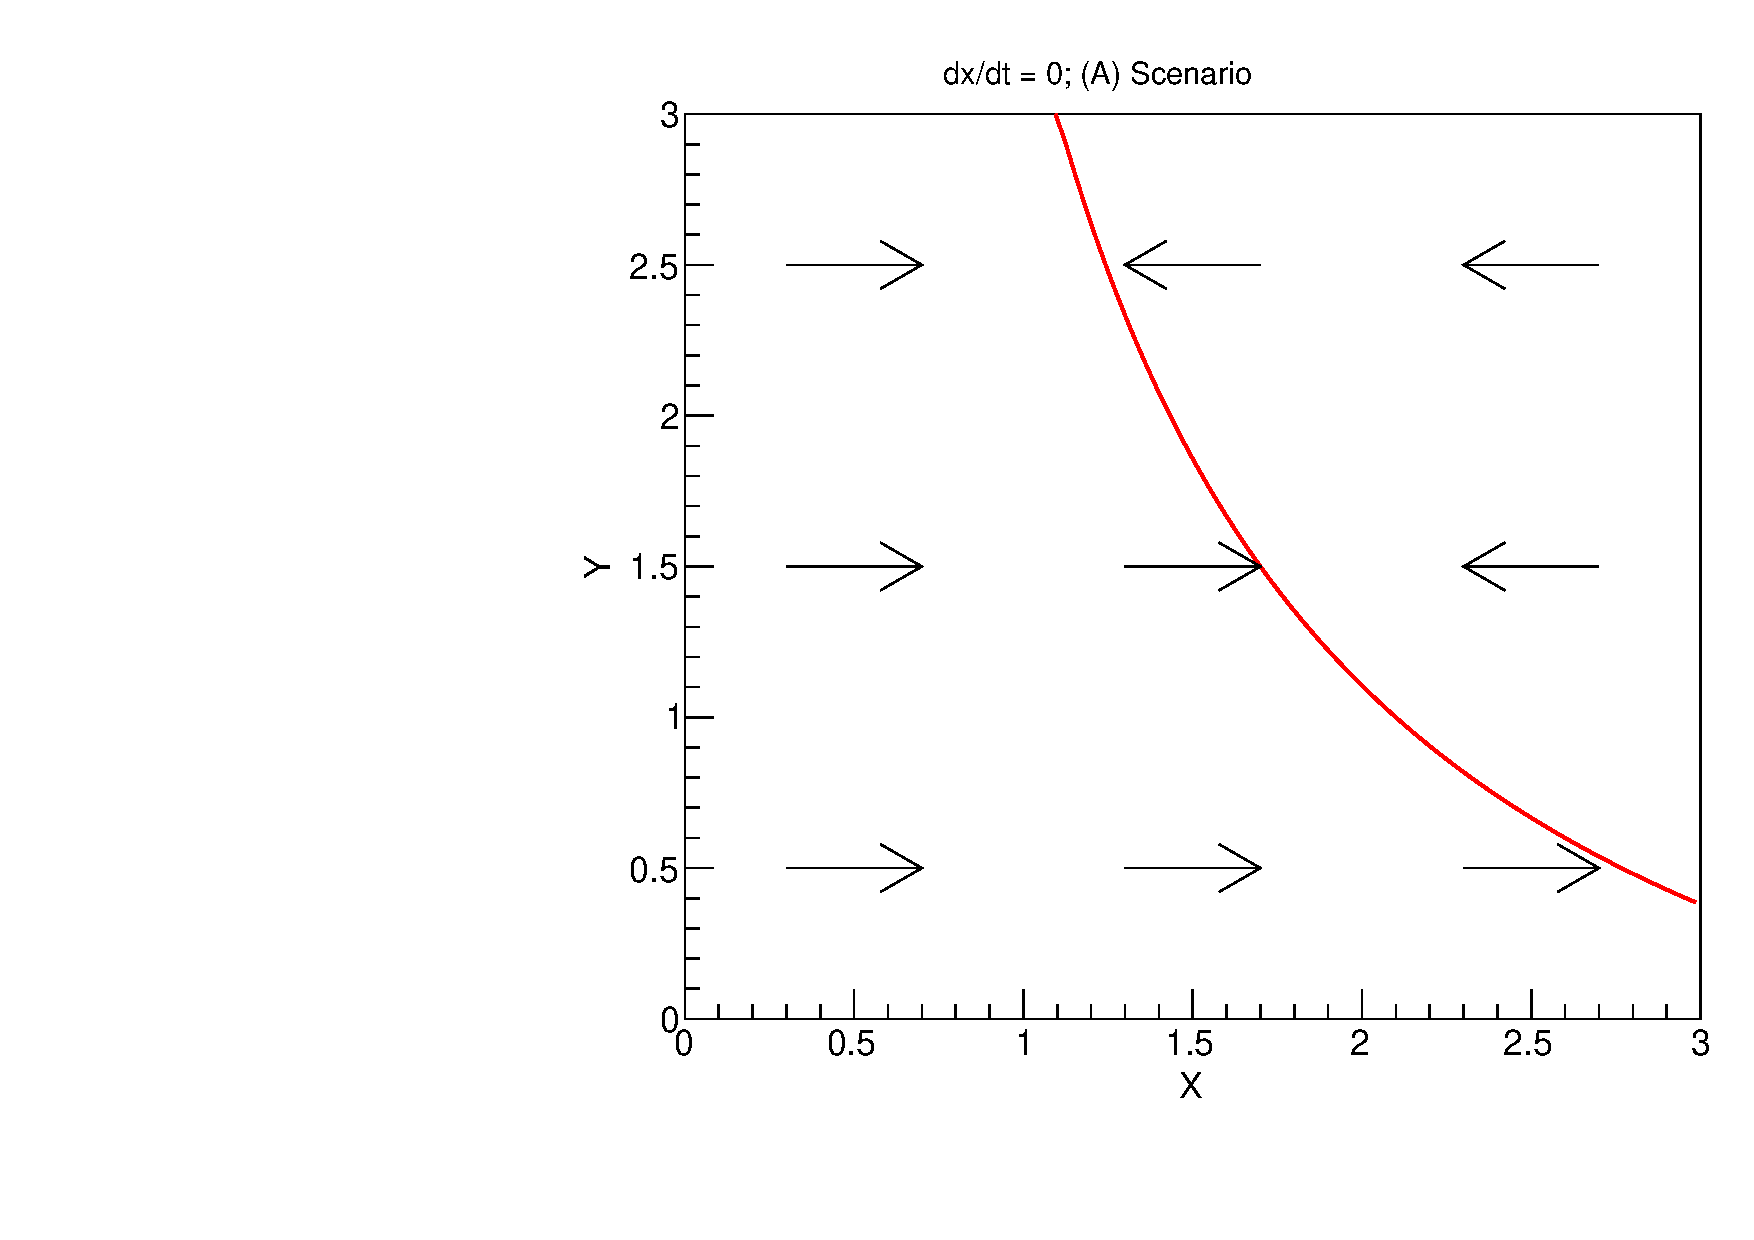
\includegraphics[width=.32\textwidth]{xDotNull1Canv.pdf} 
    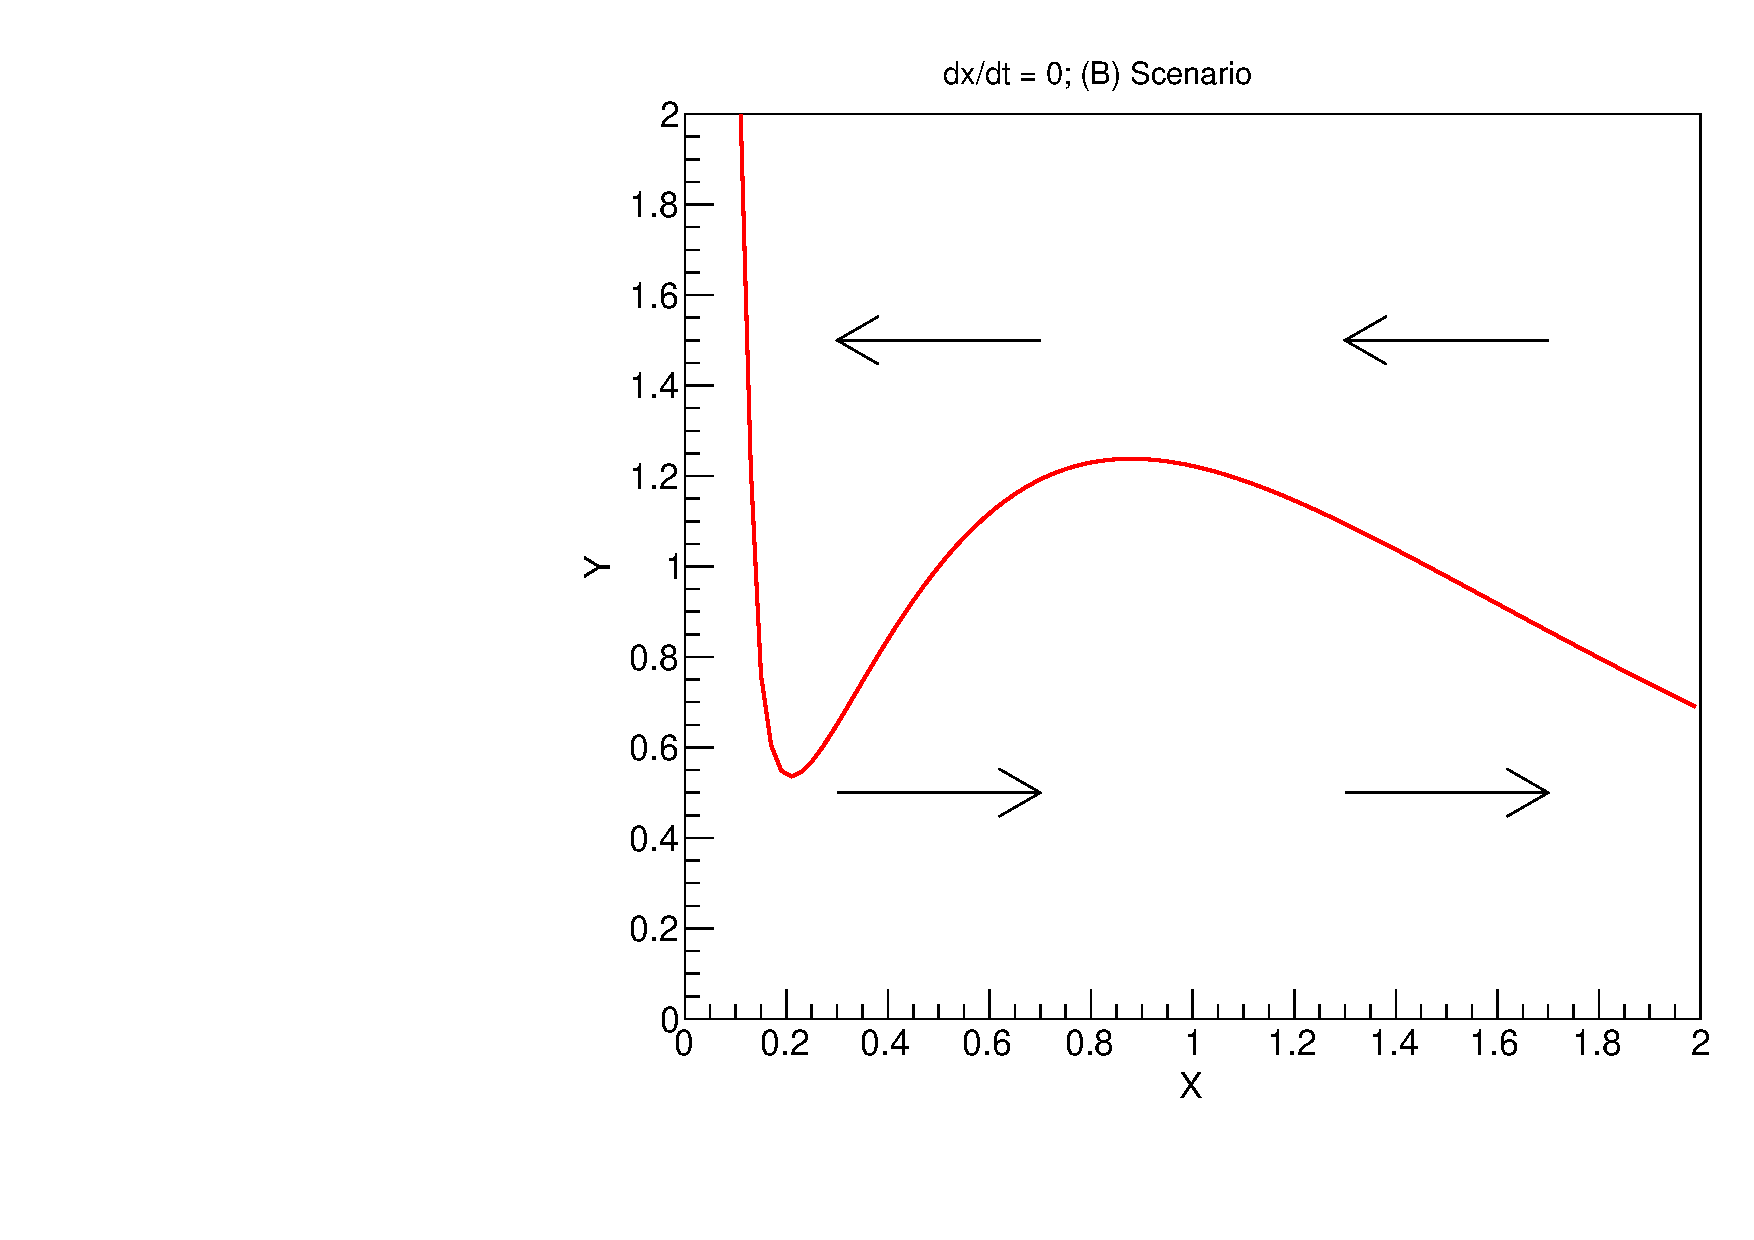
\includegraphics[width=.32\textwidth]{xDotNull2Canv.pdf}
    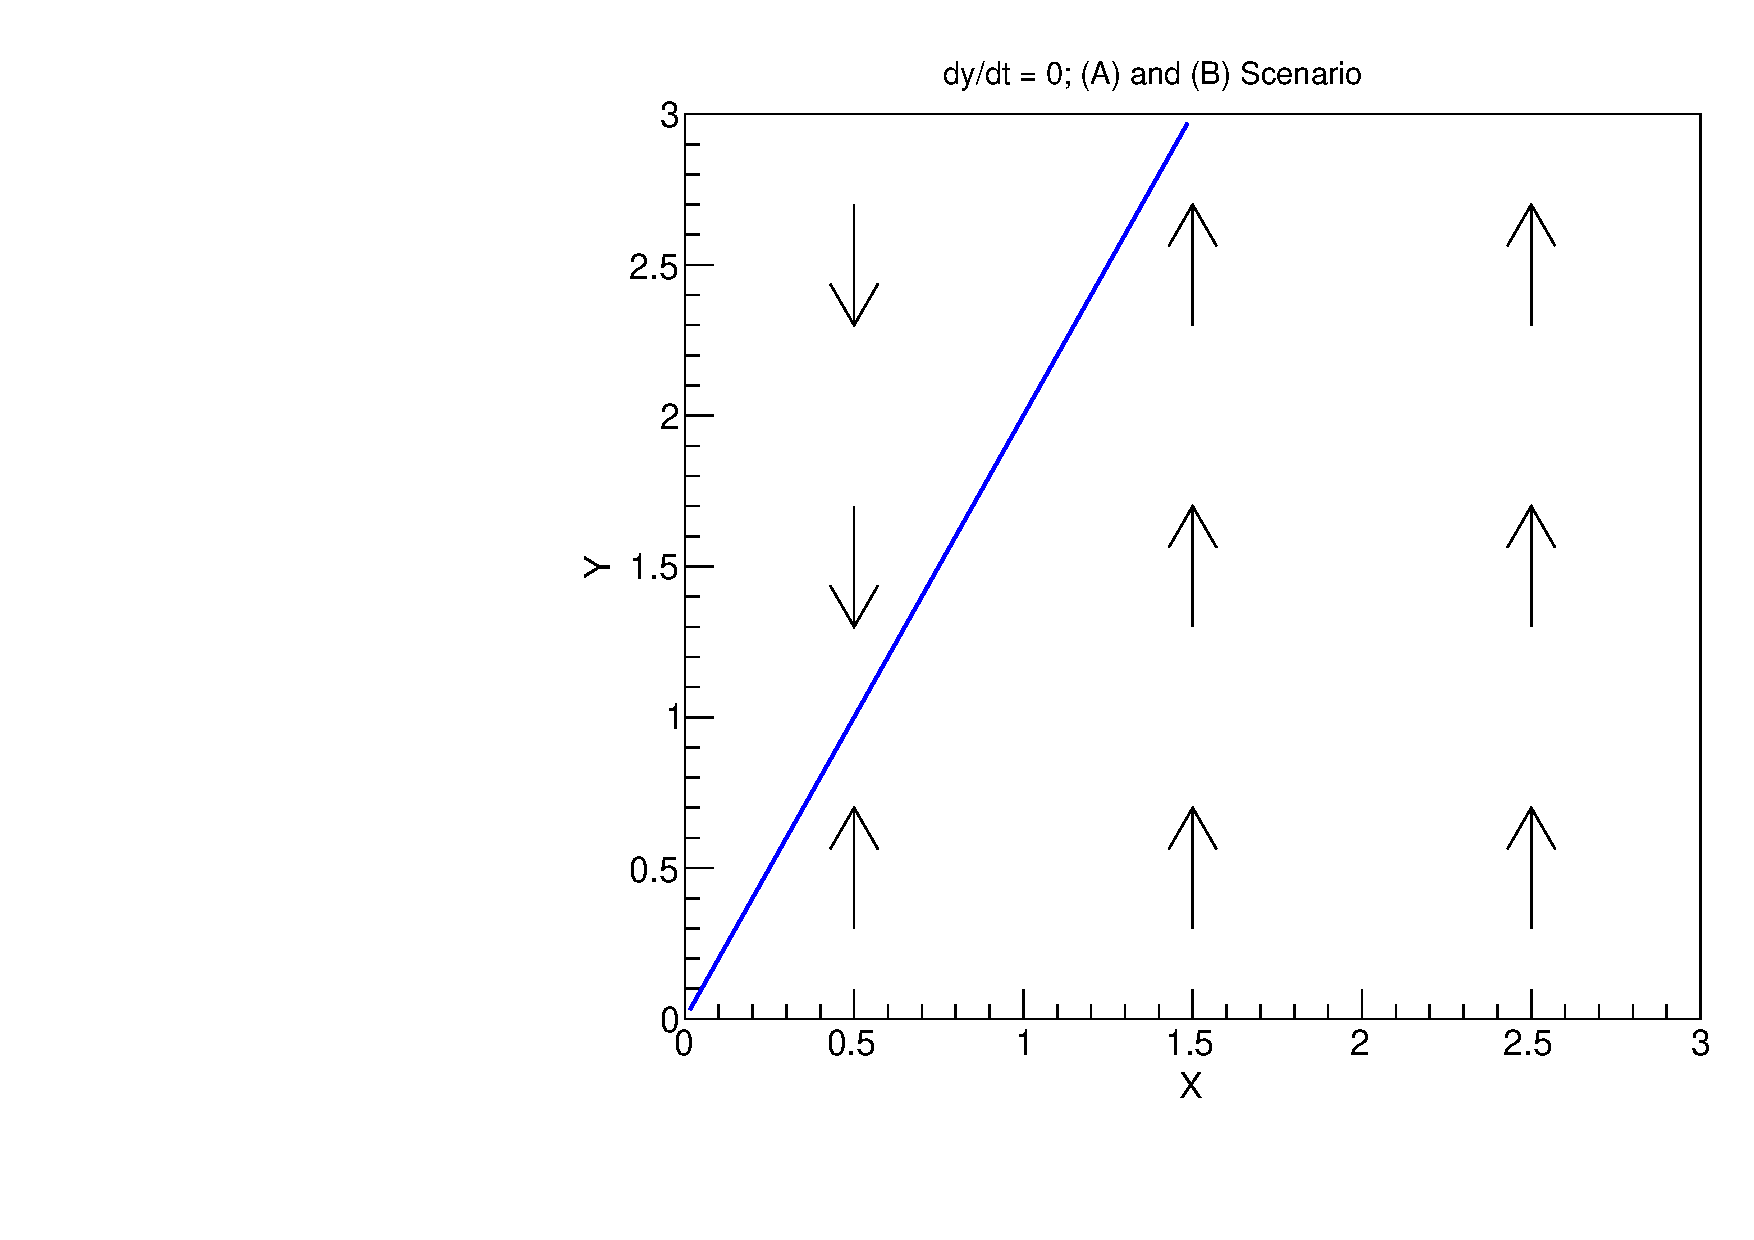
\includegraphics[width=.32\textwidth]{yDotNullCanv.pdf}
    \caption{Left: dx/dt = 0 nullcline for scenario (A). Middle: dx/dt = 0 nullcline for scenario (B). Right: dy/dt = 0 nullcline for scenarios (A) and (B). Note in all cases we are using the dimensionless units of 1c, or x,y relative to concentrations $A_{i}$.}
    \label{}
\end{figure}

\begin{figure}[H]
    \centering
    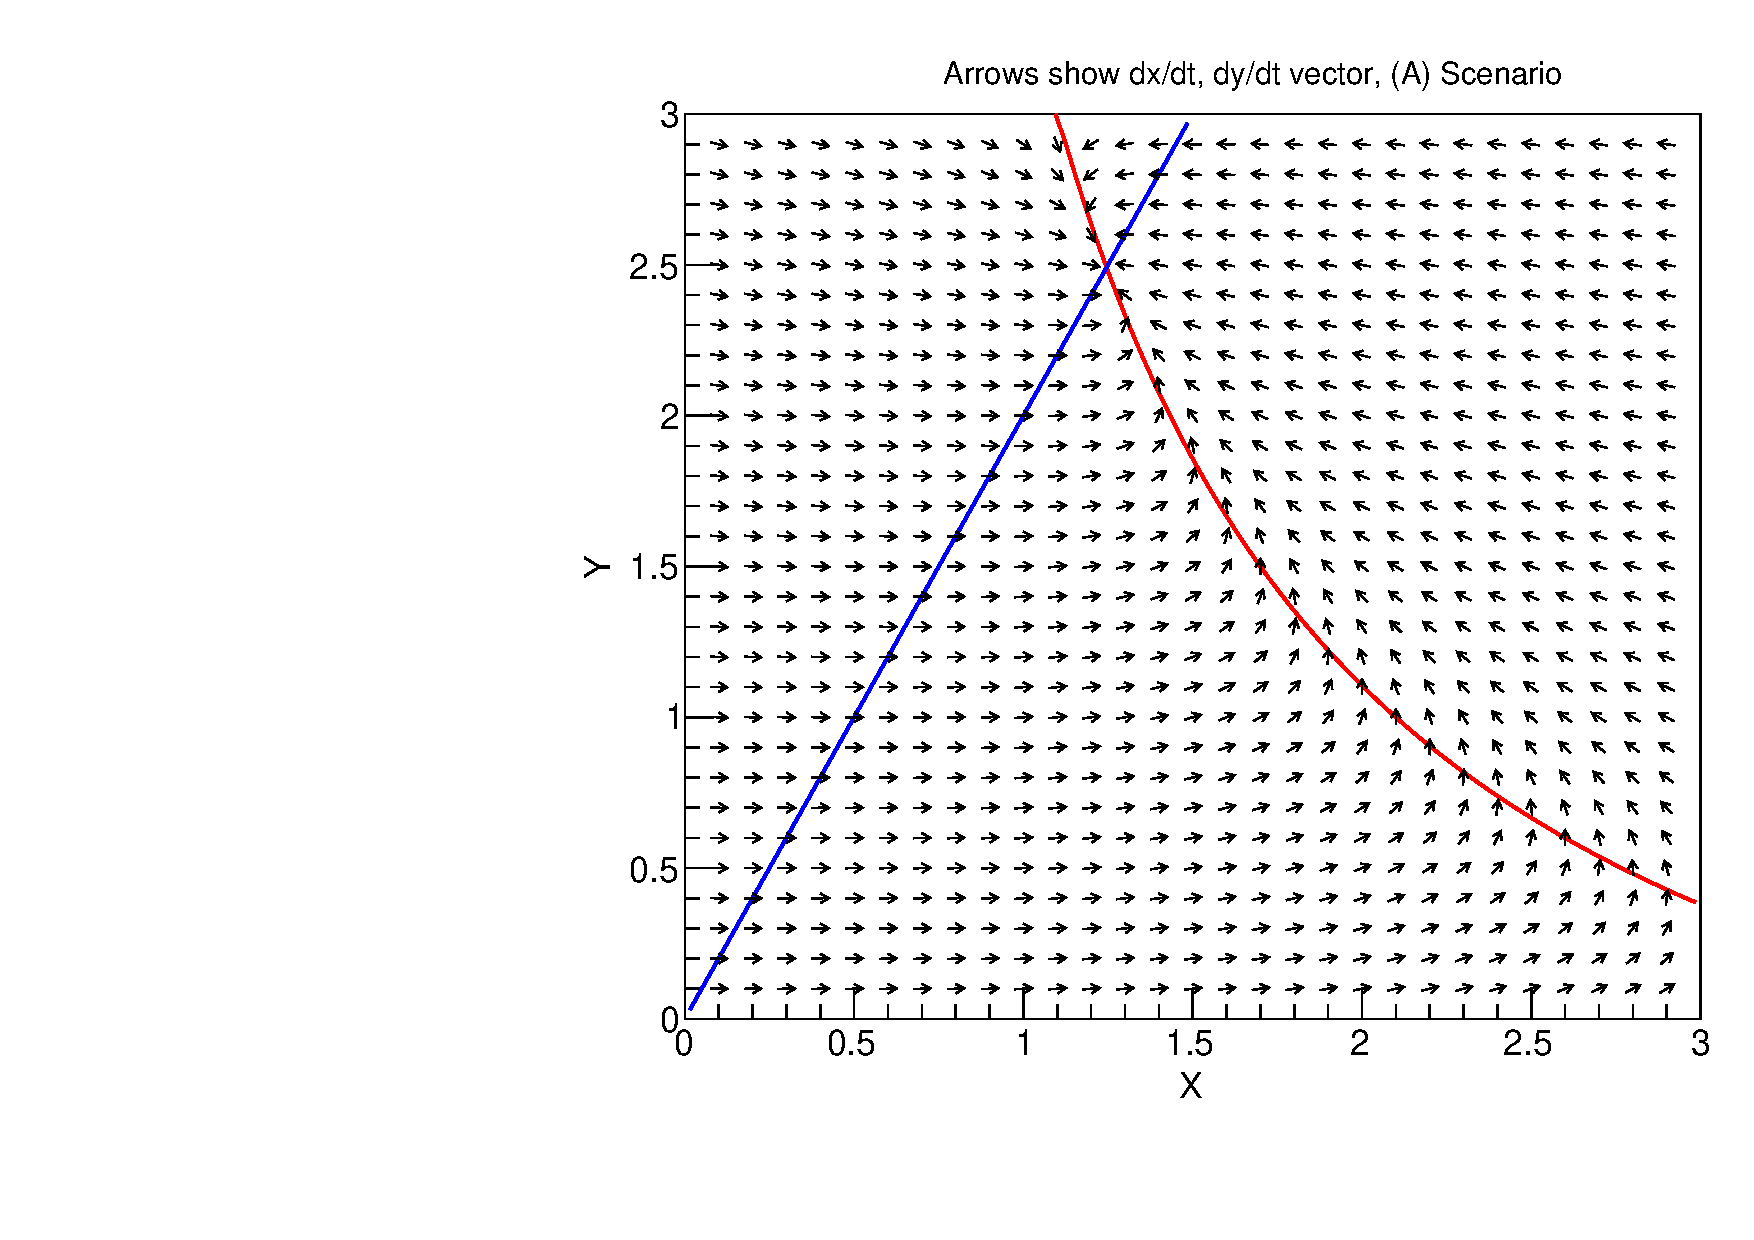
\includegraphics[width=.49\textwidth]{canv1.pdf} 
    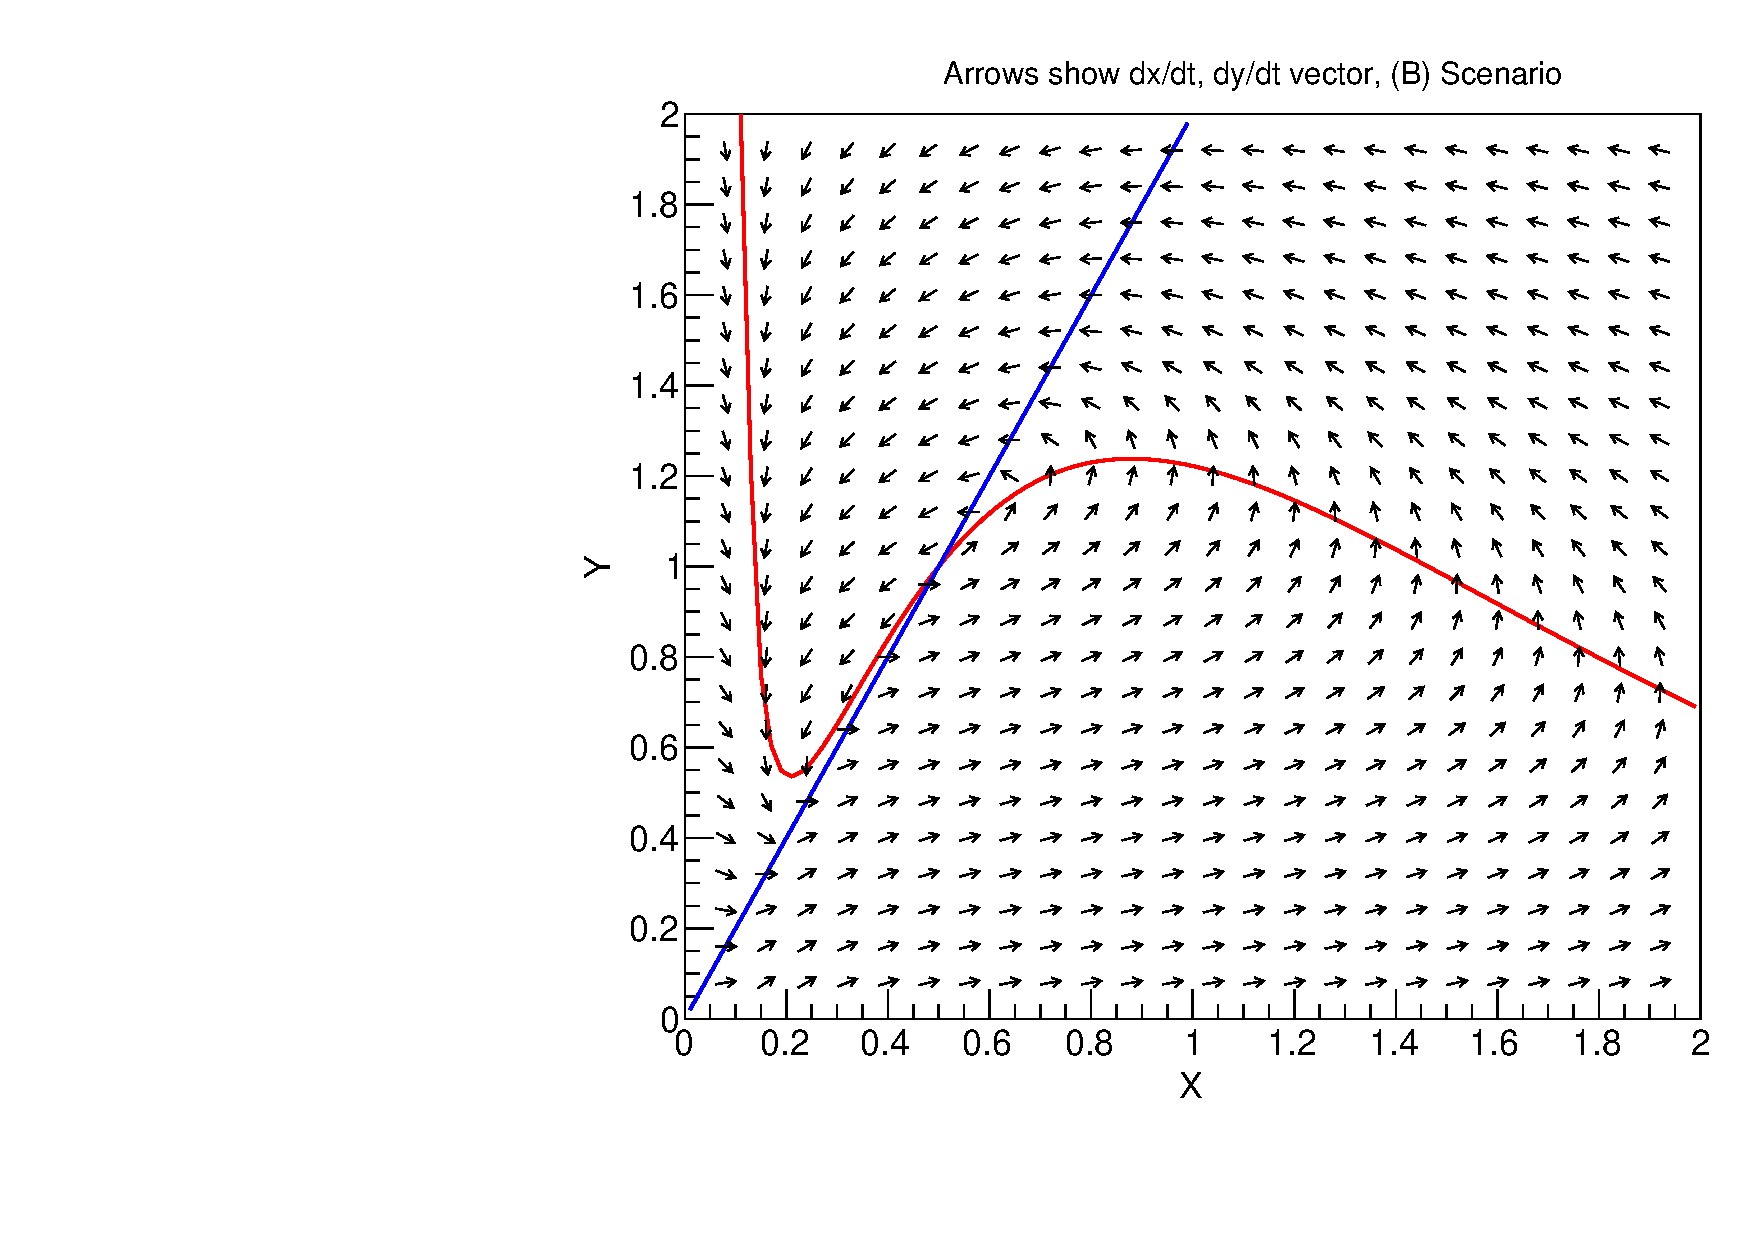
\includegraphics[width=.49\textwidth]{canv2.pdf}
    \caption{Left: Direction of motion at each point in x-y for scenario (A) and given parameter set. Fixed point is stable. Right: Direction of motion at each point in x-y for scenario (B) and given parameter set. Fixed point is unstable. Again note all x,y are in dimensionless units.}
    \label{}
\end{figure}

\section{1.f.2-3}
The following set of plots correspond to analysis of system (B) in problem 1, Circadian Clocks. Code can be found at https://github.com/cfmcginn/SystBio/tree/master/HW3. C++ and ROOT needed to run. A directory containing the set of pdfs used in this document is available at the git repository, along with the .tex used to create this, if wanted individually. From this set of plots, choice of $\gamma_{X} < 25/7$ shows rapid decay to some stable value. In contrast, choices of $\gamma_{X} > 25/7$ show sustained oscillations. Period and amplitude of oscillations in the steady state region both depend on choice of $gamma_{X}$ for fixed initial conditions, but both show asymtotic behavior as gamma is taken arbitrarily high or close to 25/7 (See figures of period, peak-to-peak height as function of $\gamma_{X}$). Note everything here is done in dimensionless units, and simulation is done with Euler-forward method with infinitessimal timesteps (such that order of magnitude changes in timescale did not significantly change results). 

Comparison with repressilator - repressilator shows a narrow frequency range (within a factor 2) with a large amplitude range (spanning at least one order magnitude) with tuned parameters. In contrast, the Circadian clock nearly spans a full order of magnitude in periodicity once it reaches stable oscillations (10.5 or so down to 1.82), while its amplitude tends to be within a factor 2 for both x and y oscillations. For tuning the periodicity of the timing, something like a Circadian clock combining positive and negative feedback is a superior choice (as is also born out in the given reference, figure 3 and figure 4). The repressilator is also a noisier, less robust oscillator than the Circadian clock.

\begin{figure}[H]
    \centering
    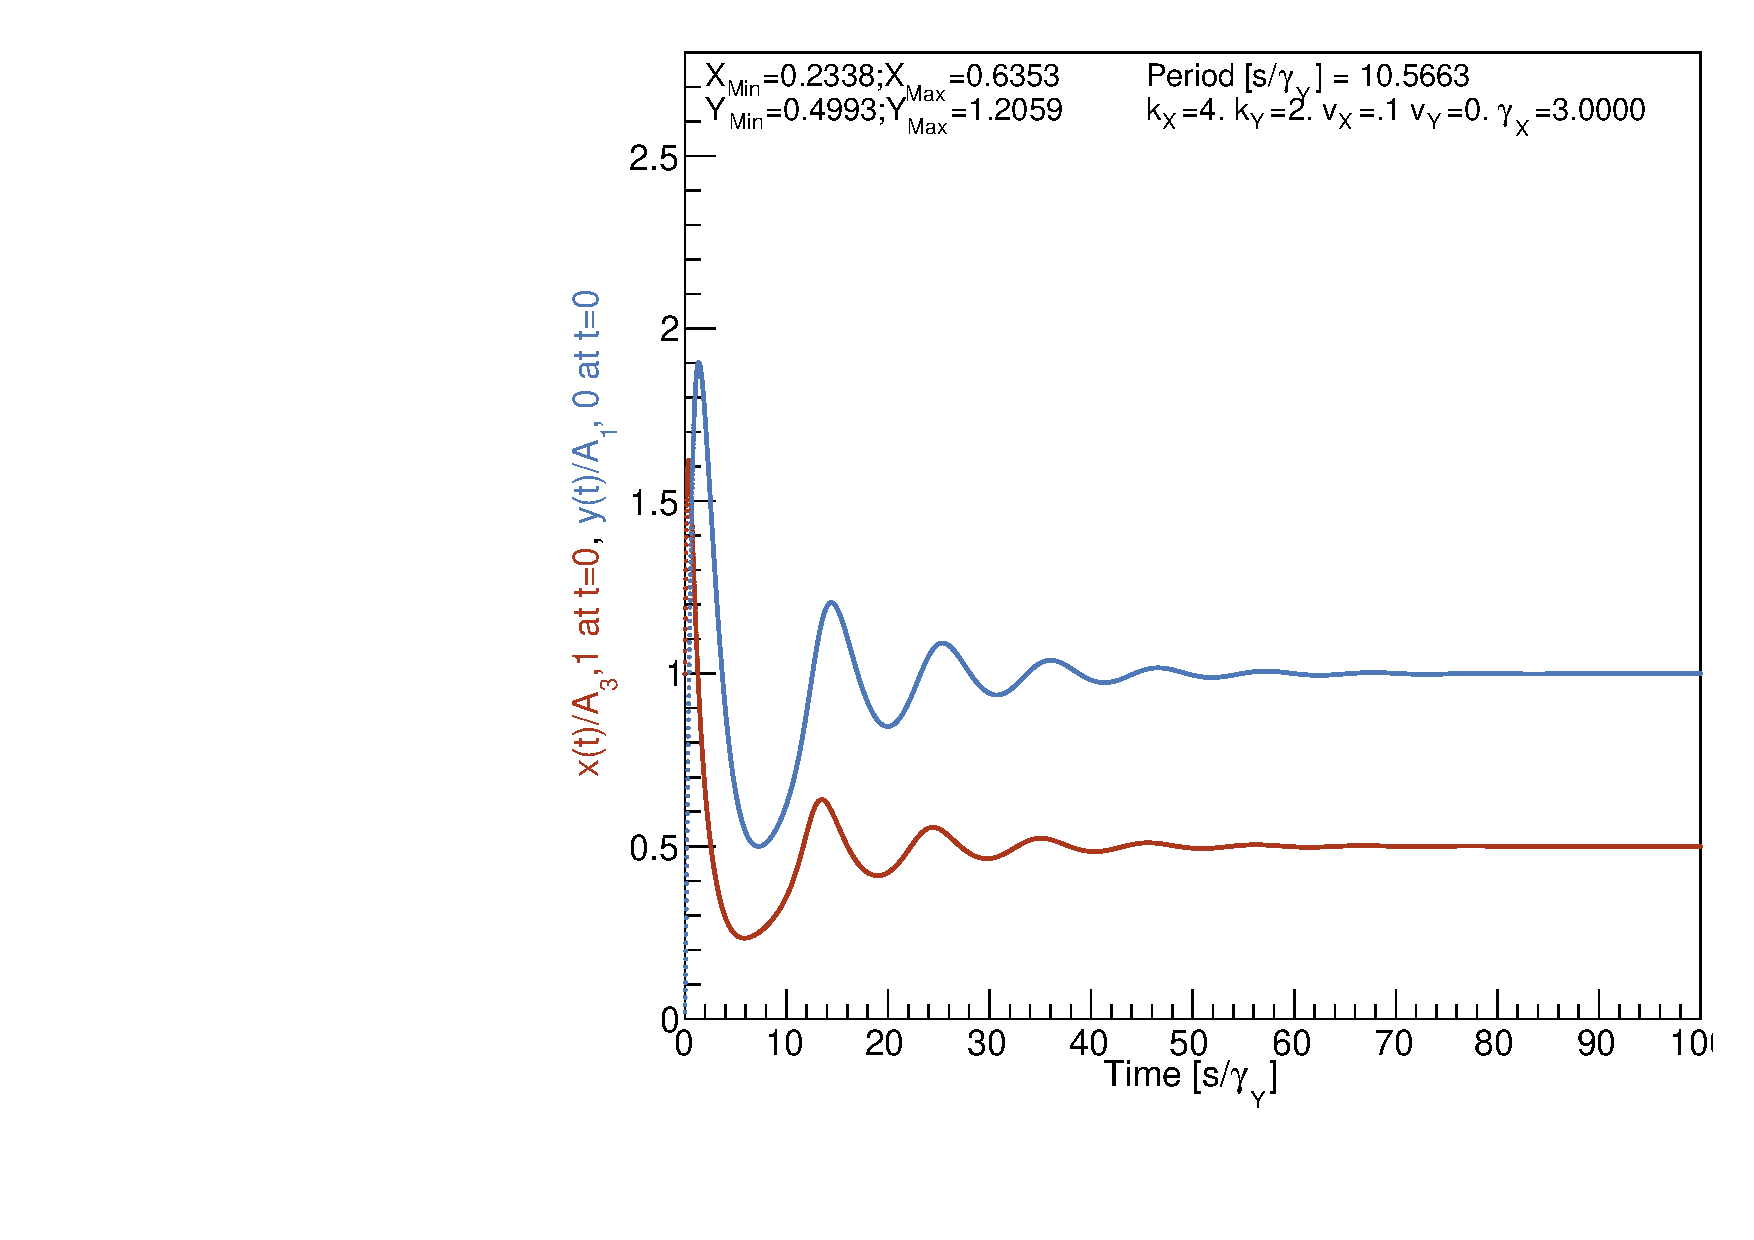
\includegraphics[width=.235\textwidth]{xy_Gamma3p0000_x1p0_y0p0_THigh100_c.pdf}
    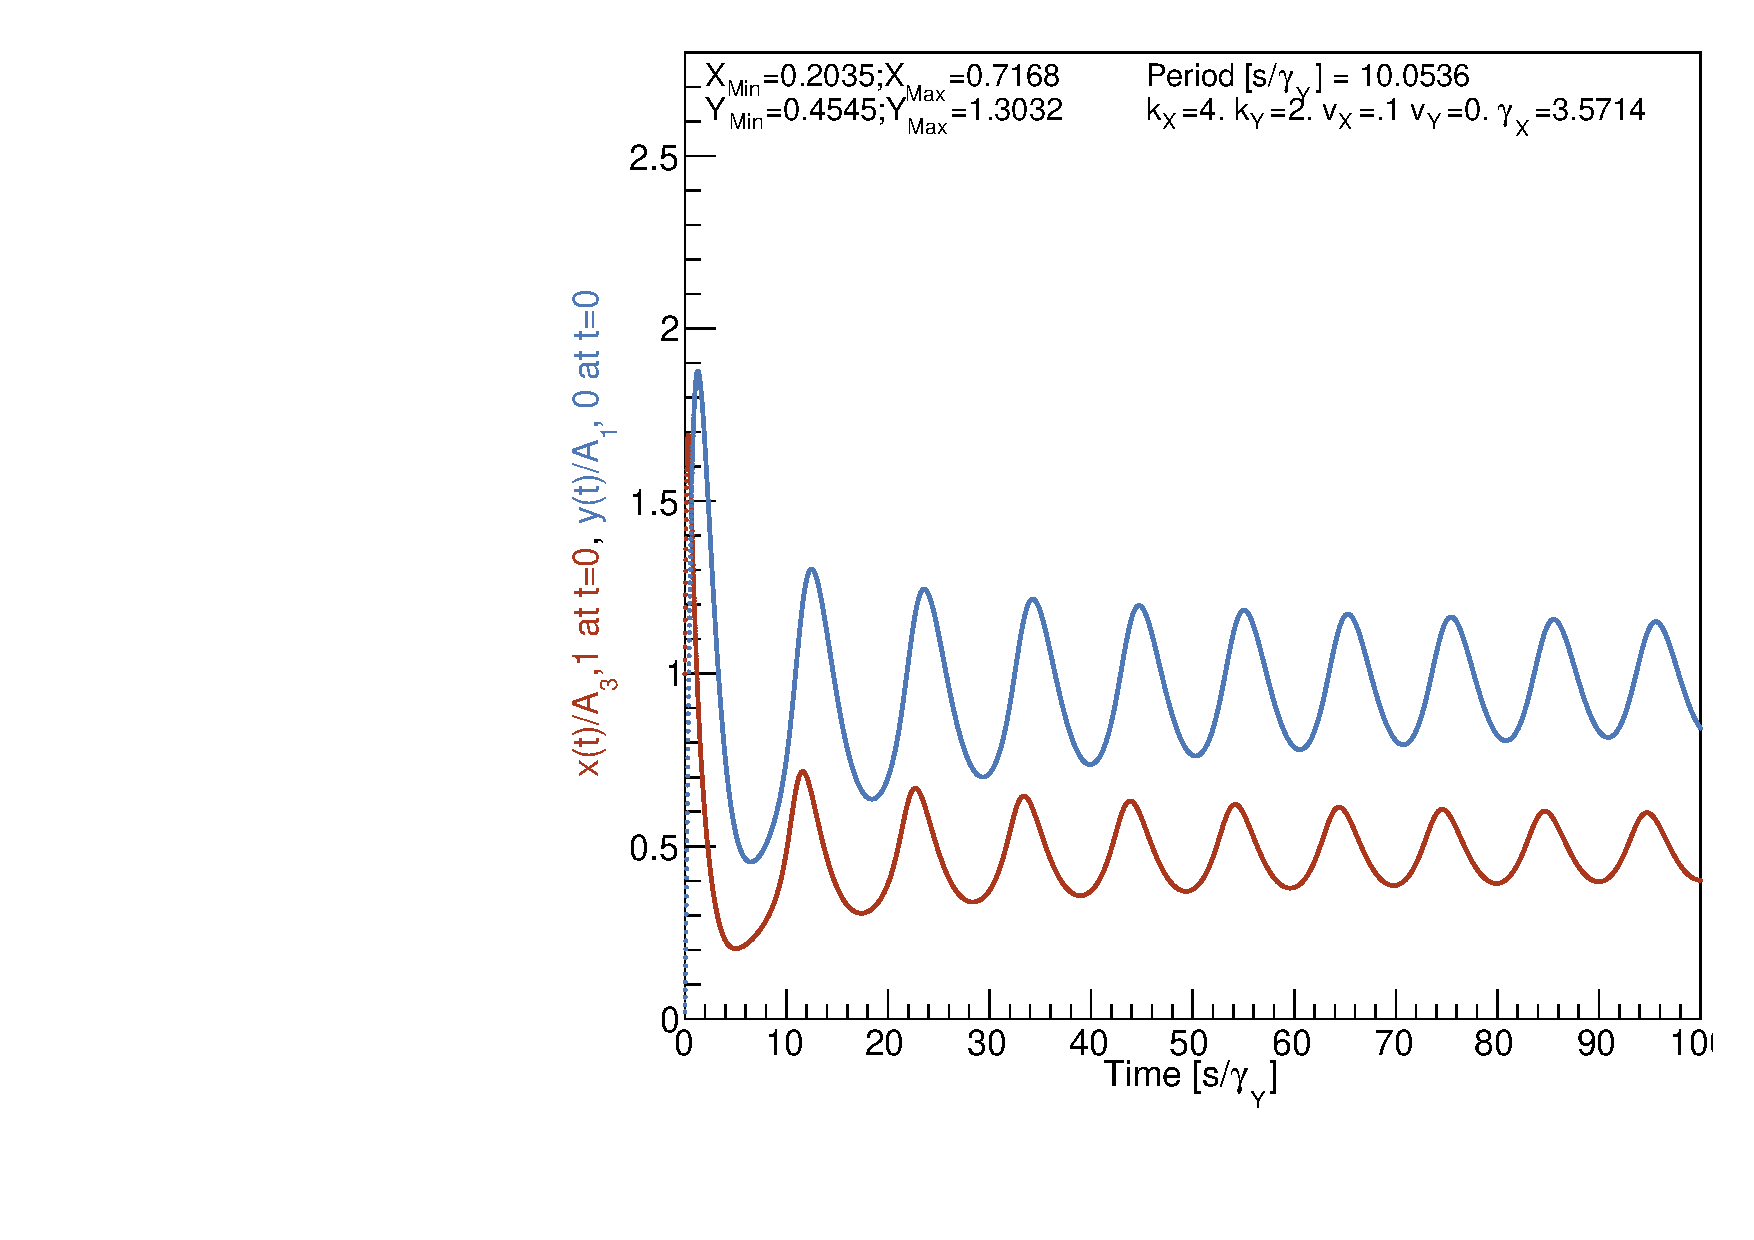
\includegraphics[width=.235\textwidth]{xy_Gamma3p5714_x1p0_y0p0_THigh100_c.pdf}
    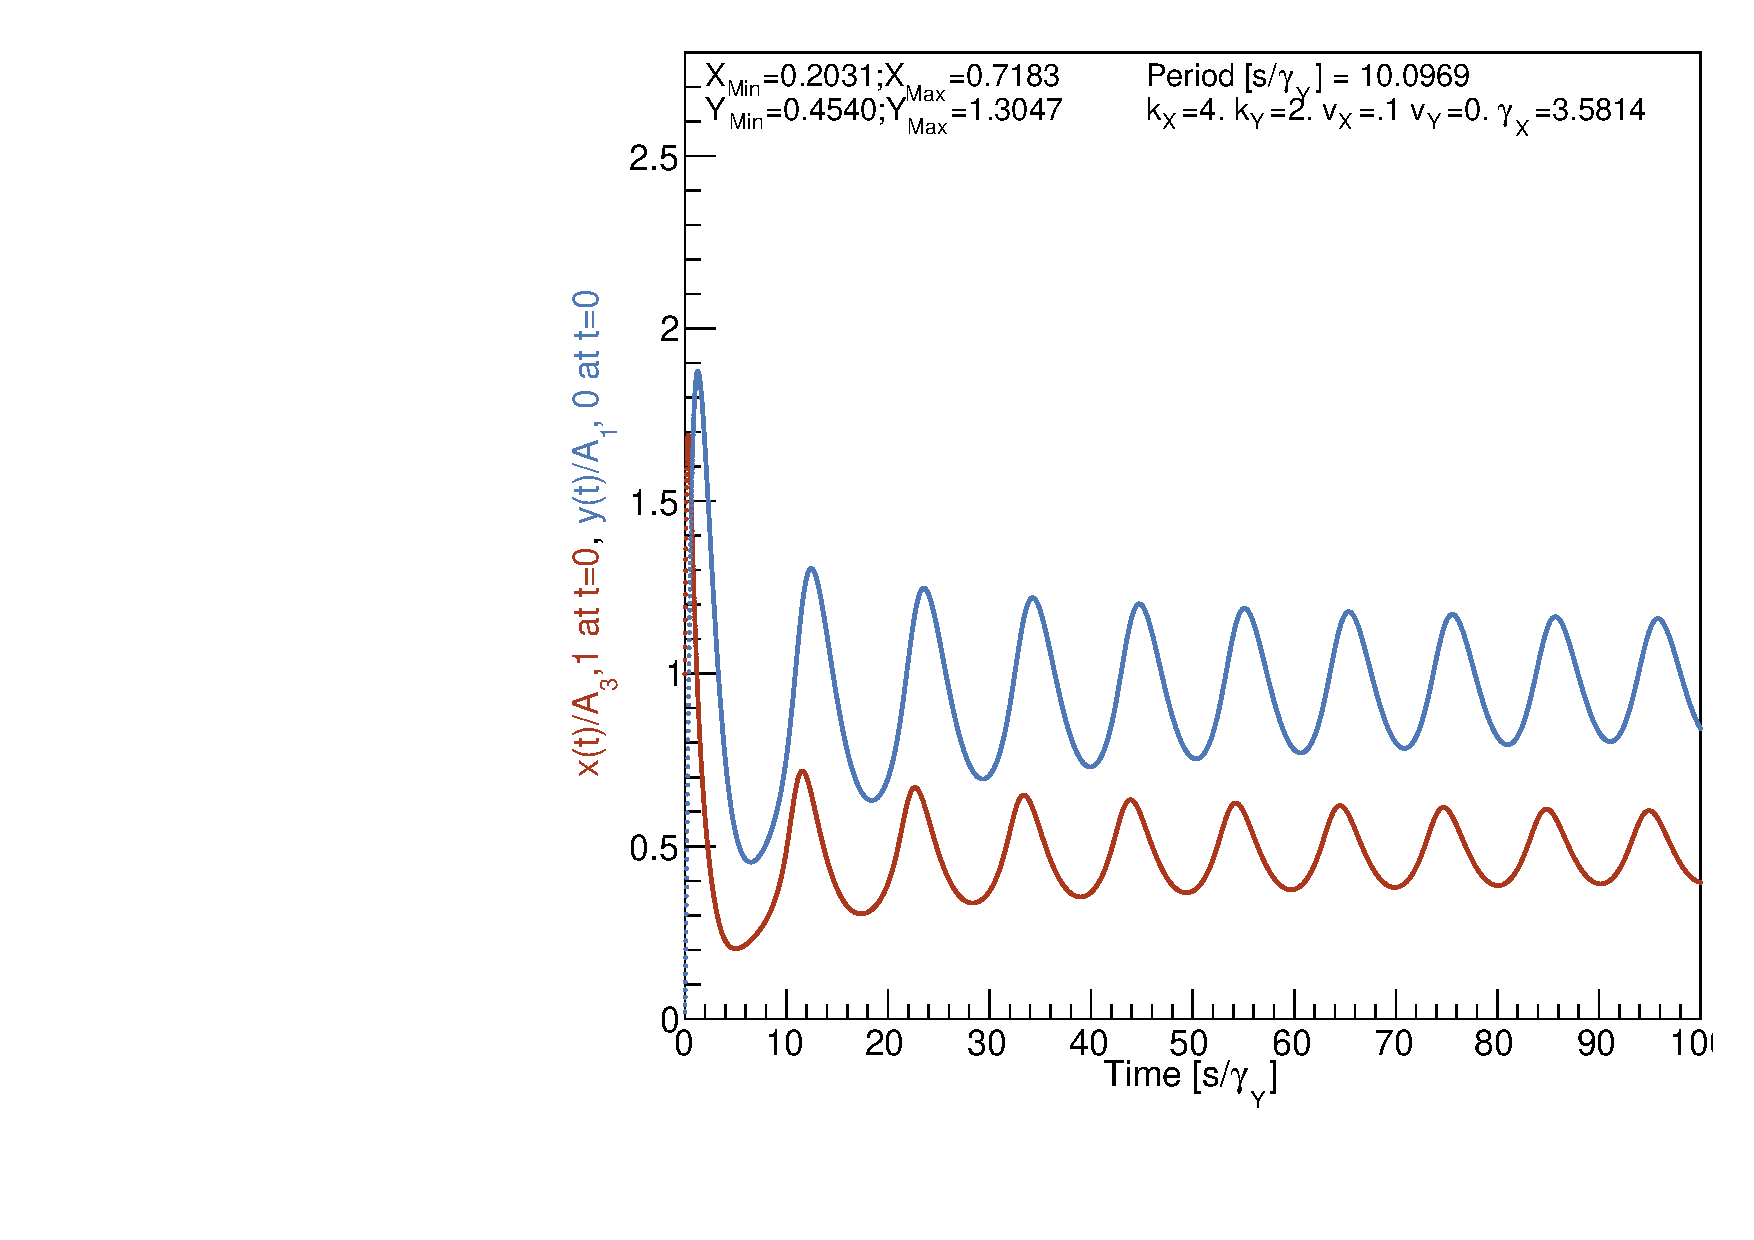
\includegraphics[width=.235\textwidth]{xy_Gamma3p5814_x1p0_y0p0_THigh100_c.pdf}
    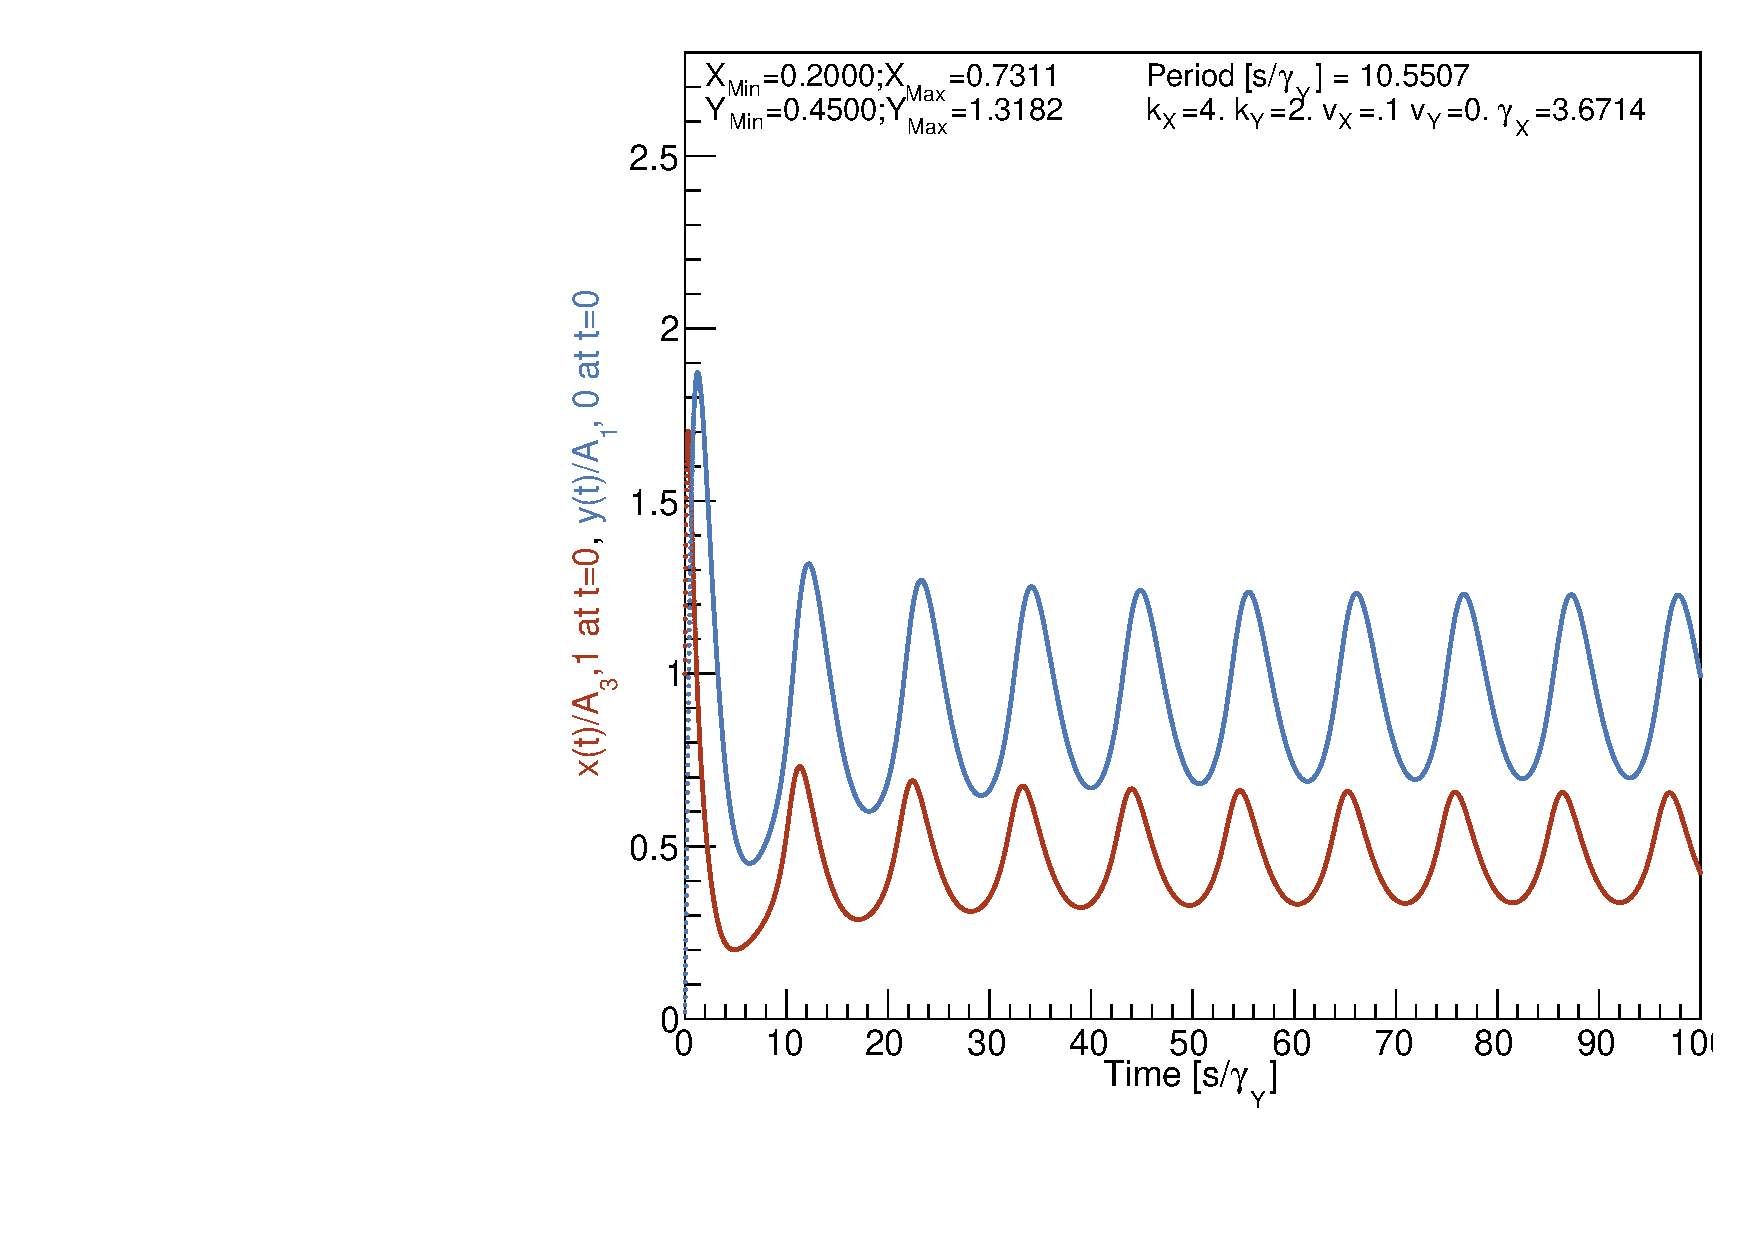
\includegraphics[width=.235\textwidth]{xy_Gamma3p6714_x1p0_y0p0_THigh100_c.pdf}
    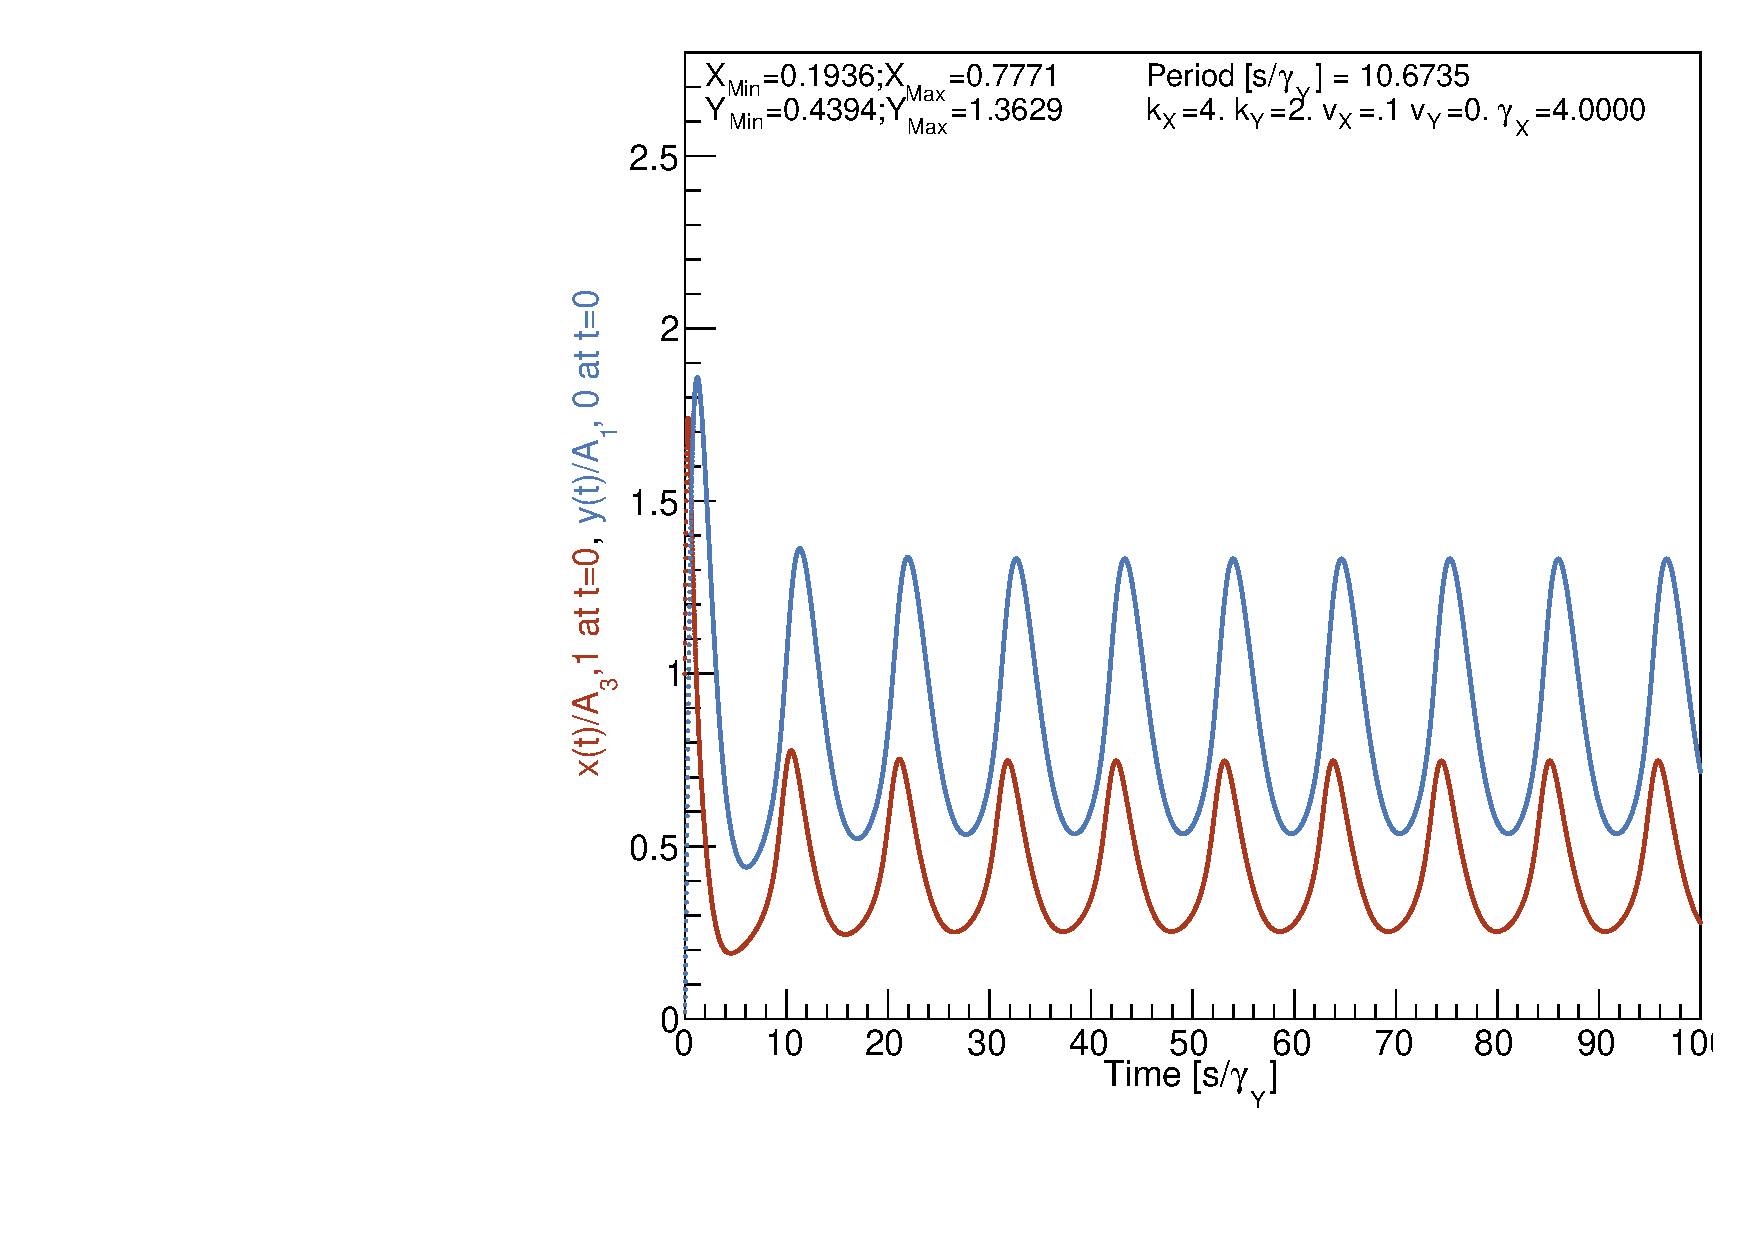
\includegraphics[width=.235\textwidth]{xy_Gamma4p0000_x1p0_y0p0_THigh100_c.pdf}
    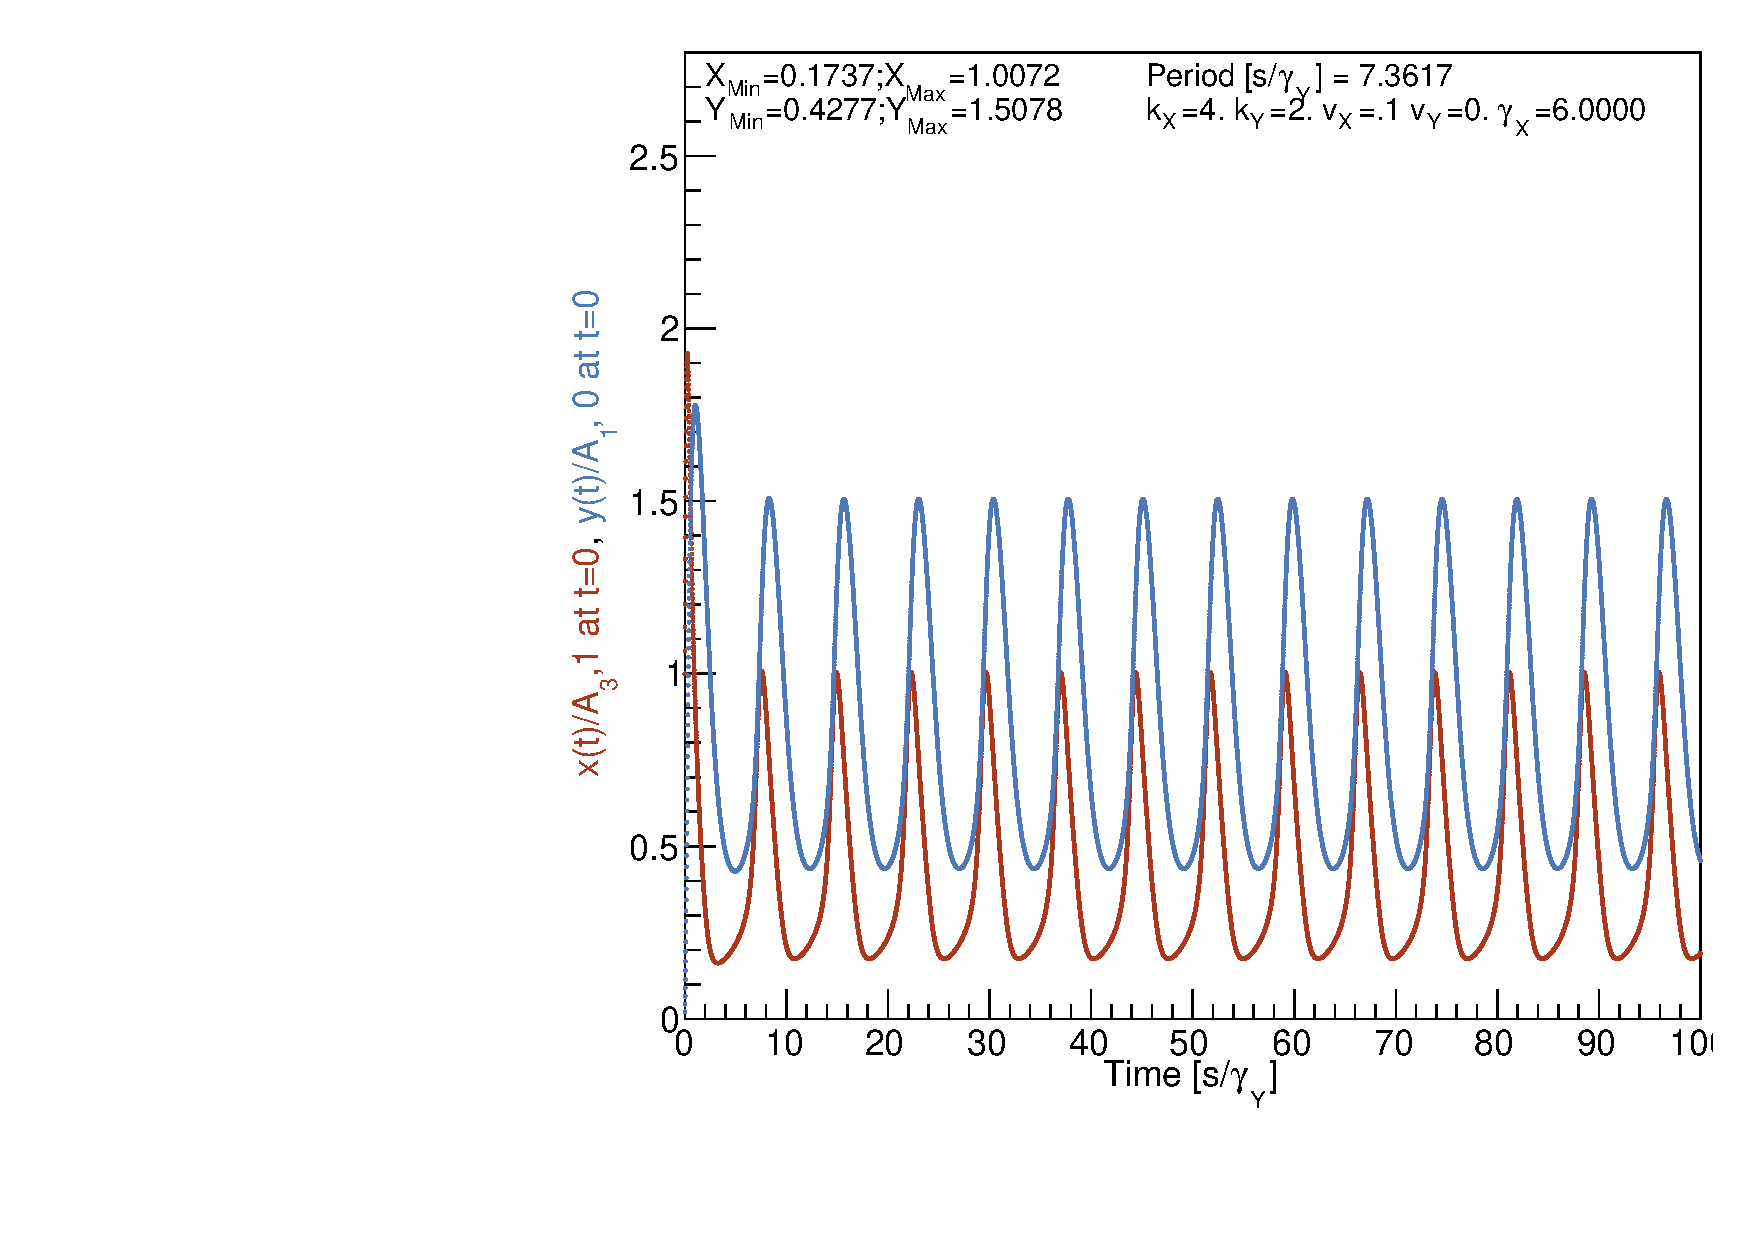
\includegraphics[width=.235\textwidth]{xy_Gamma6p0000_x1p0_y0p0_THigh100_c.pdf}
    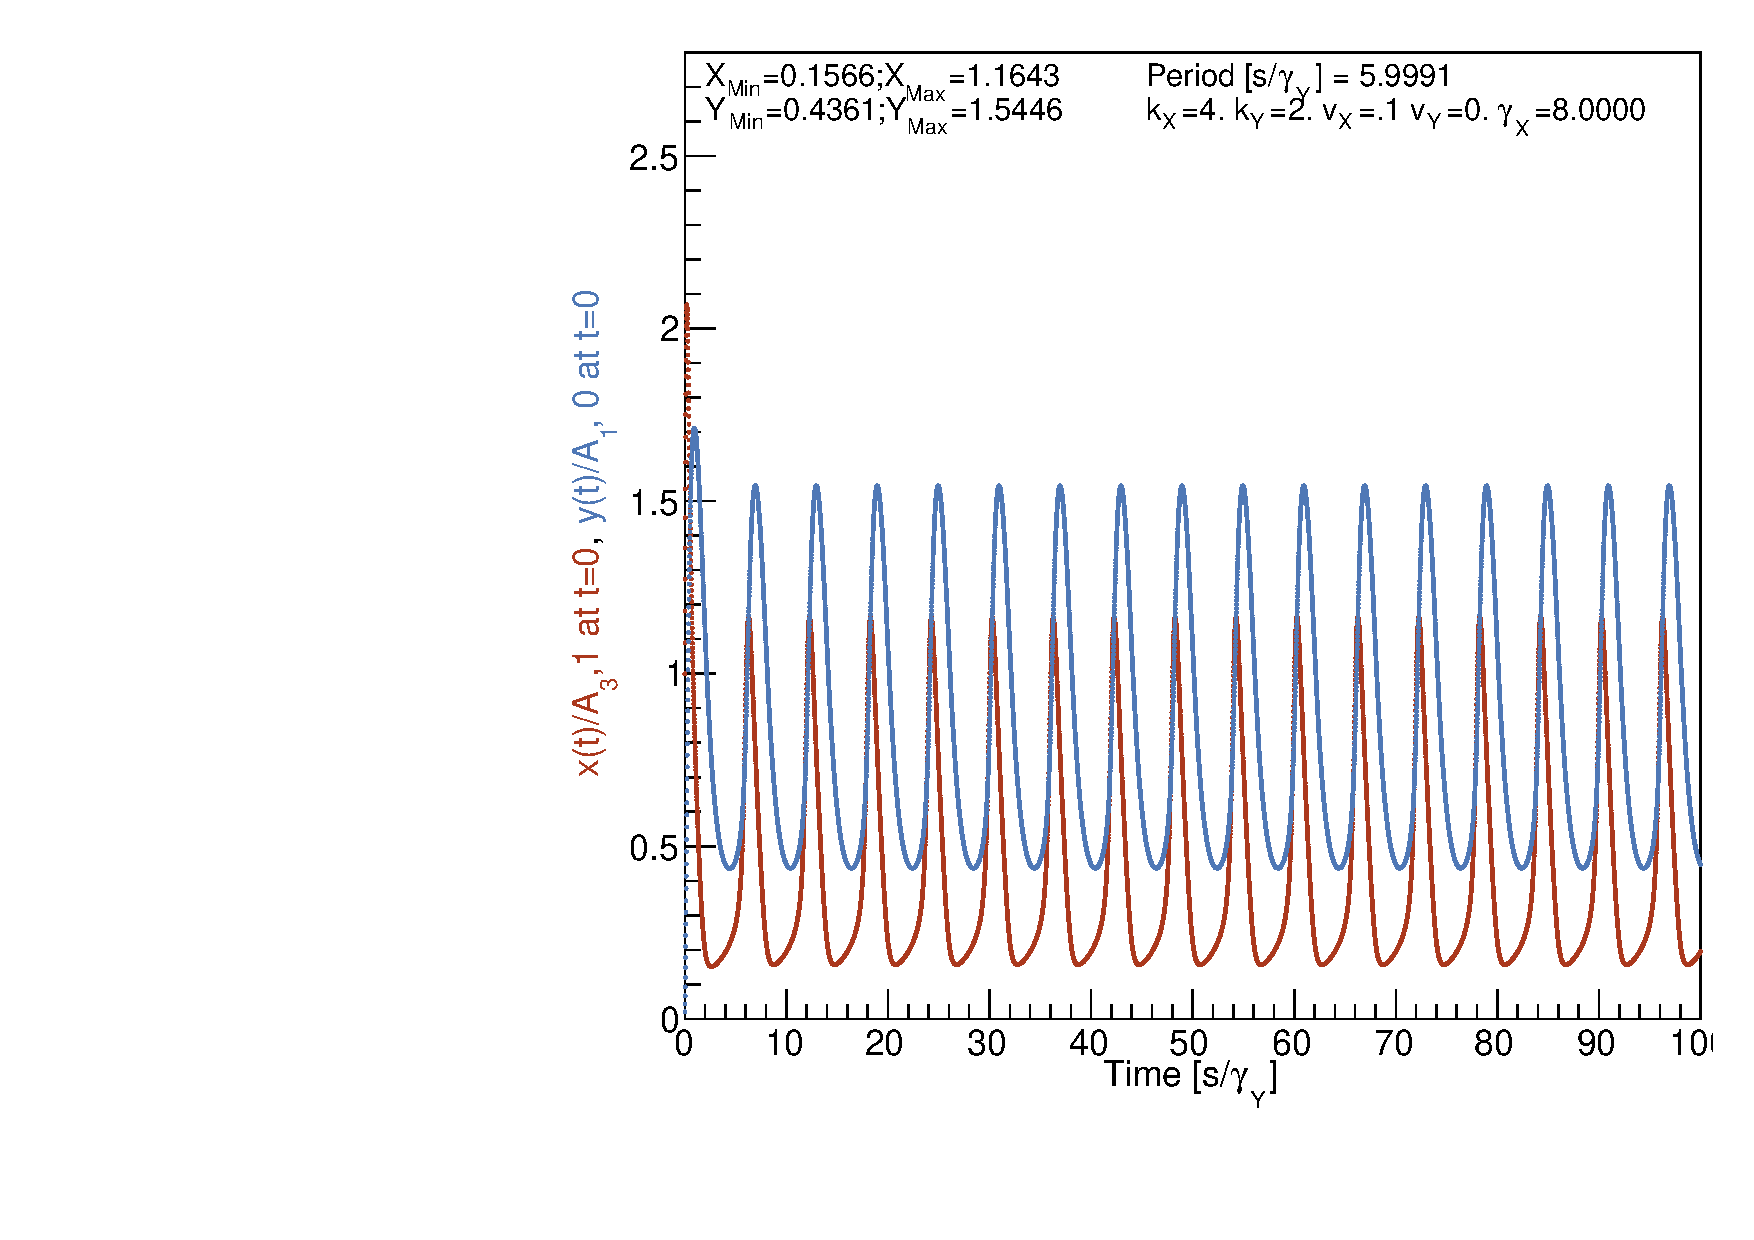
\includegraphics[width=.235\textwidth]{xy_Gamma8p0000_x1p0_y0p0_THigh100_c.pdf}
    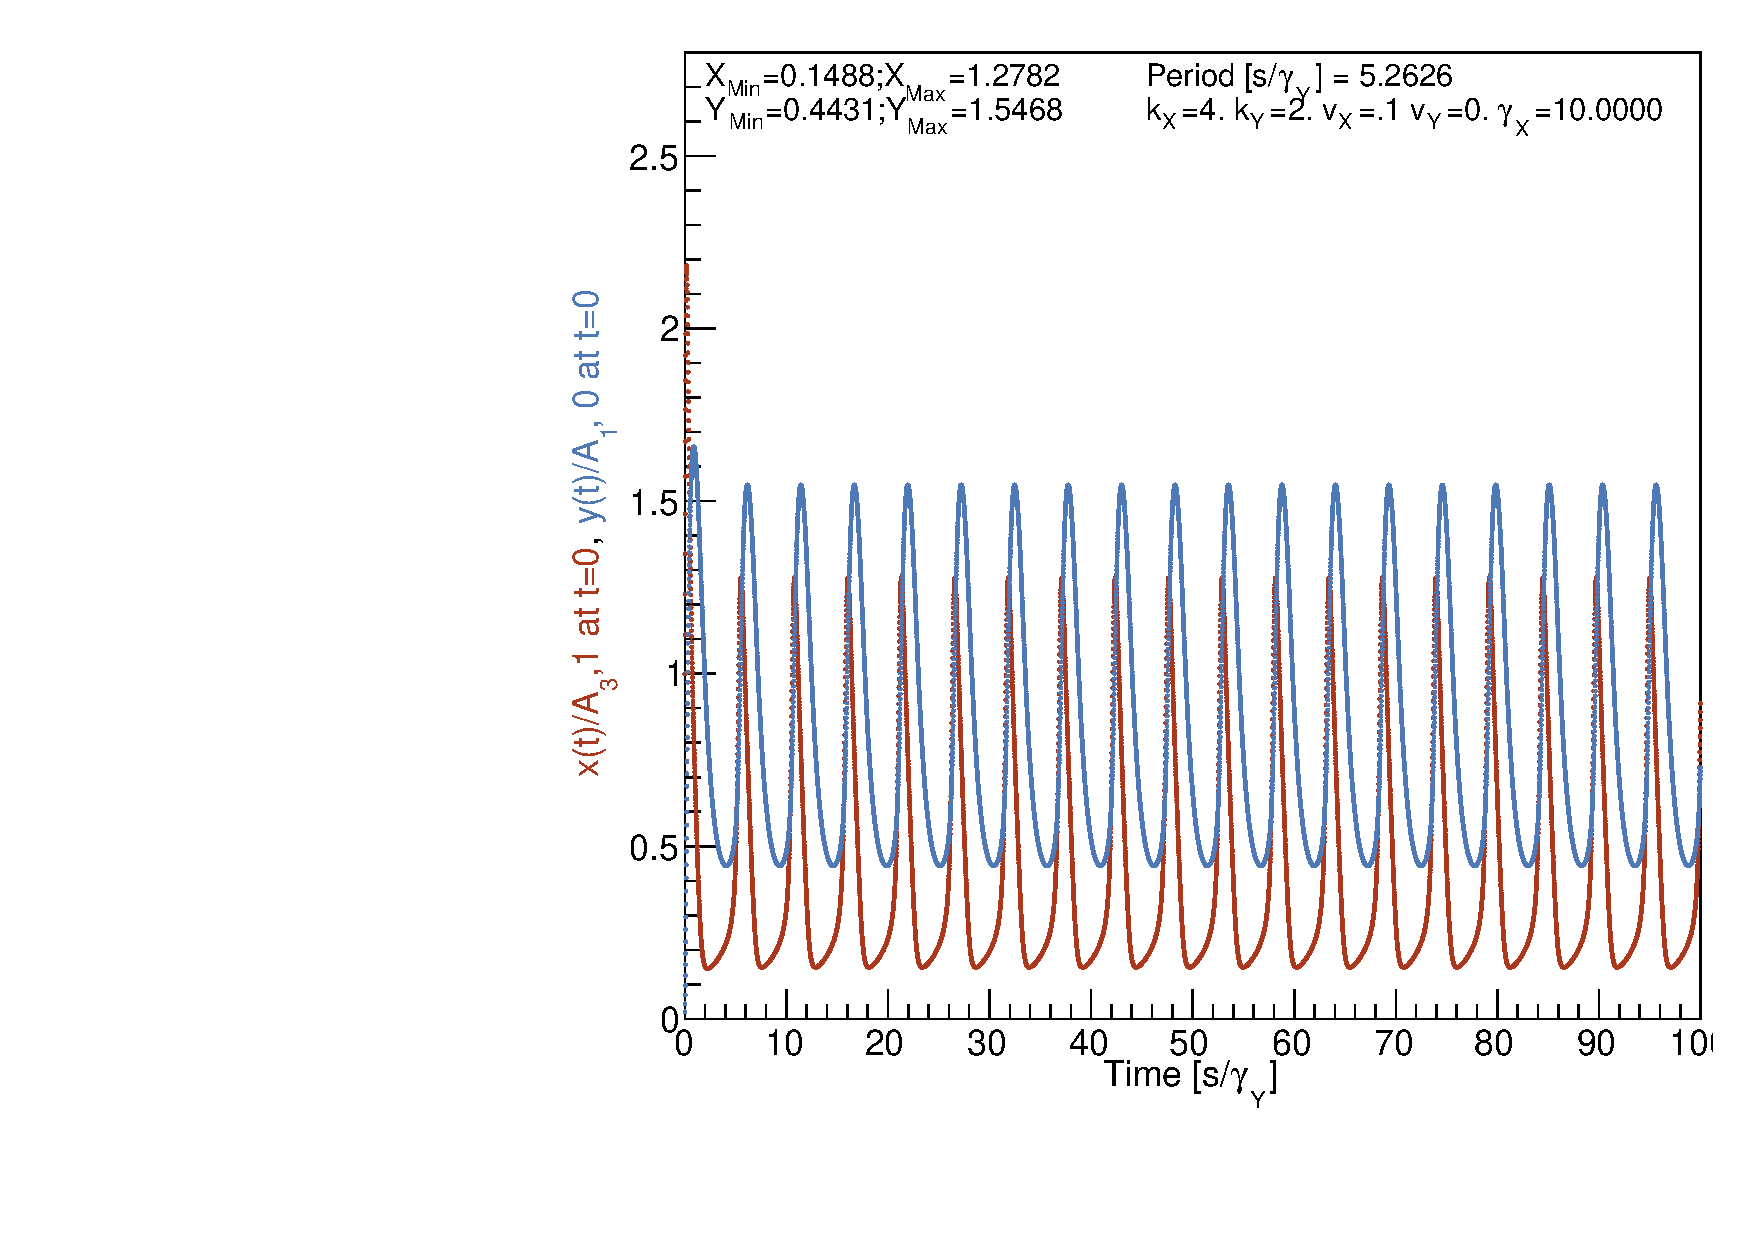
\includegraphics[width=.235\textwidth]{xy_Gamma10p0000_x1p0_y0p0_THigh100_c.pdf}
    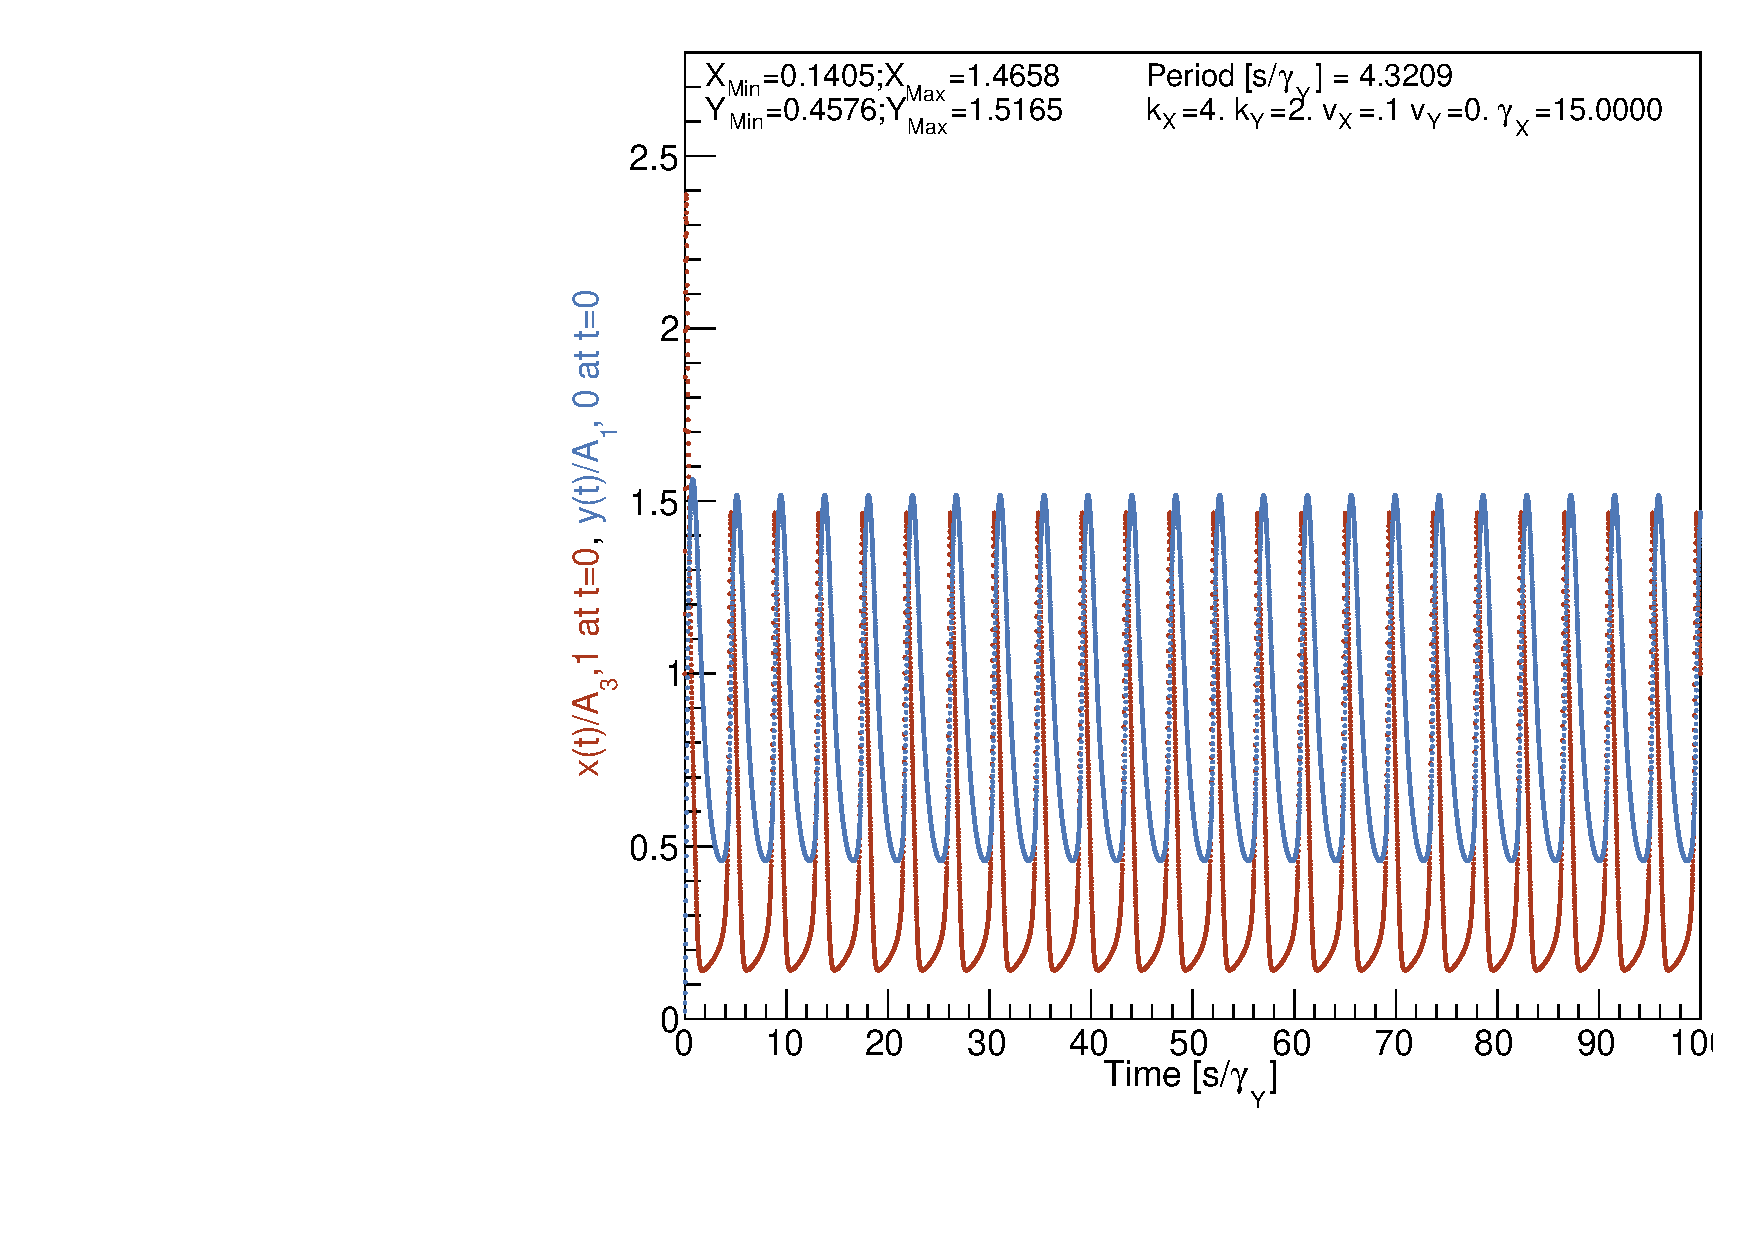
\includegraphics[width=.235\textwidth]{xy_Gamma15p0000_x1p0_y0p0_THigh100_c.pdf}
    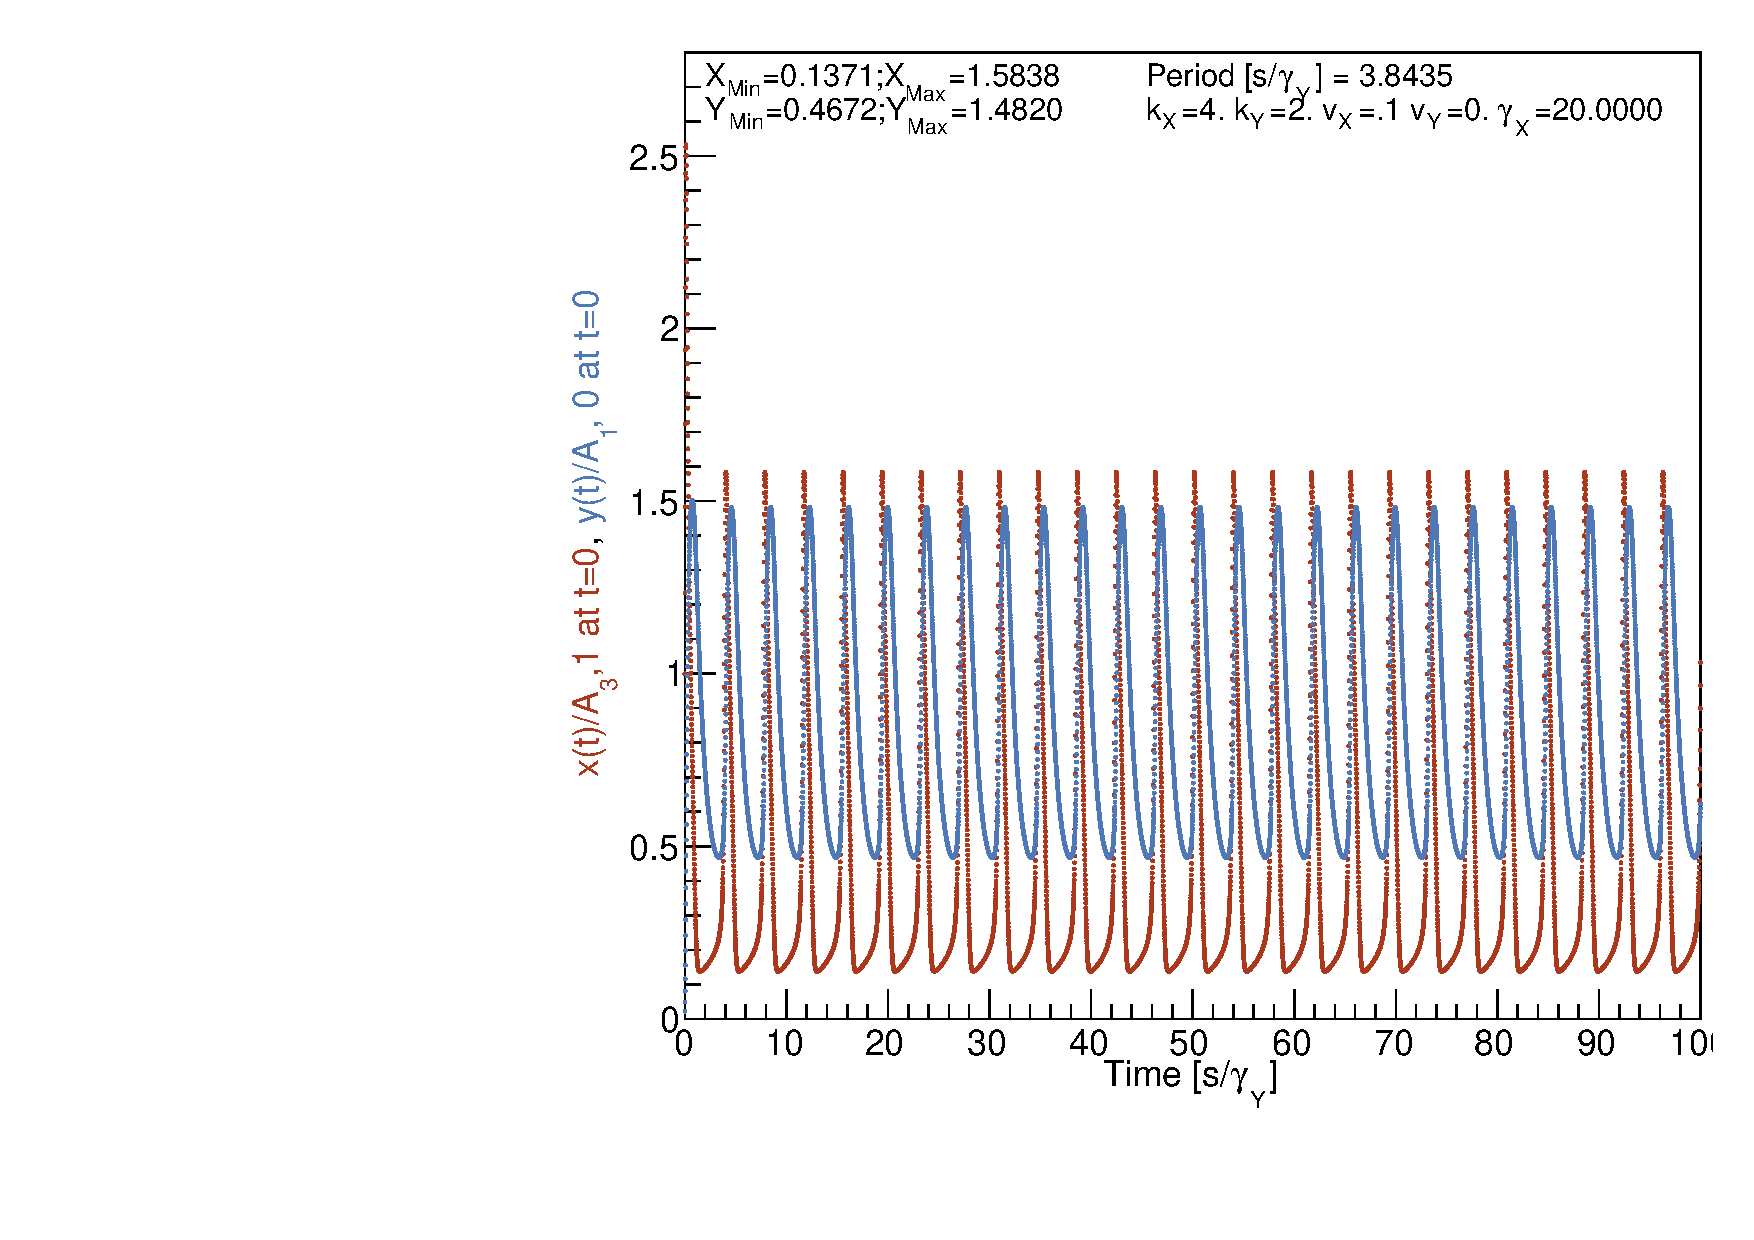
\includegraphics[width=.235\textwidth]{xy_Gamma20p0000_x1p0_y0p0_THigh100_c.pdf}
    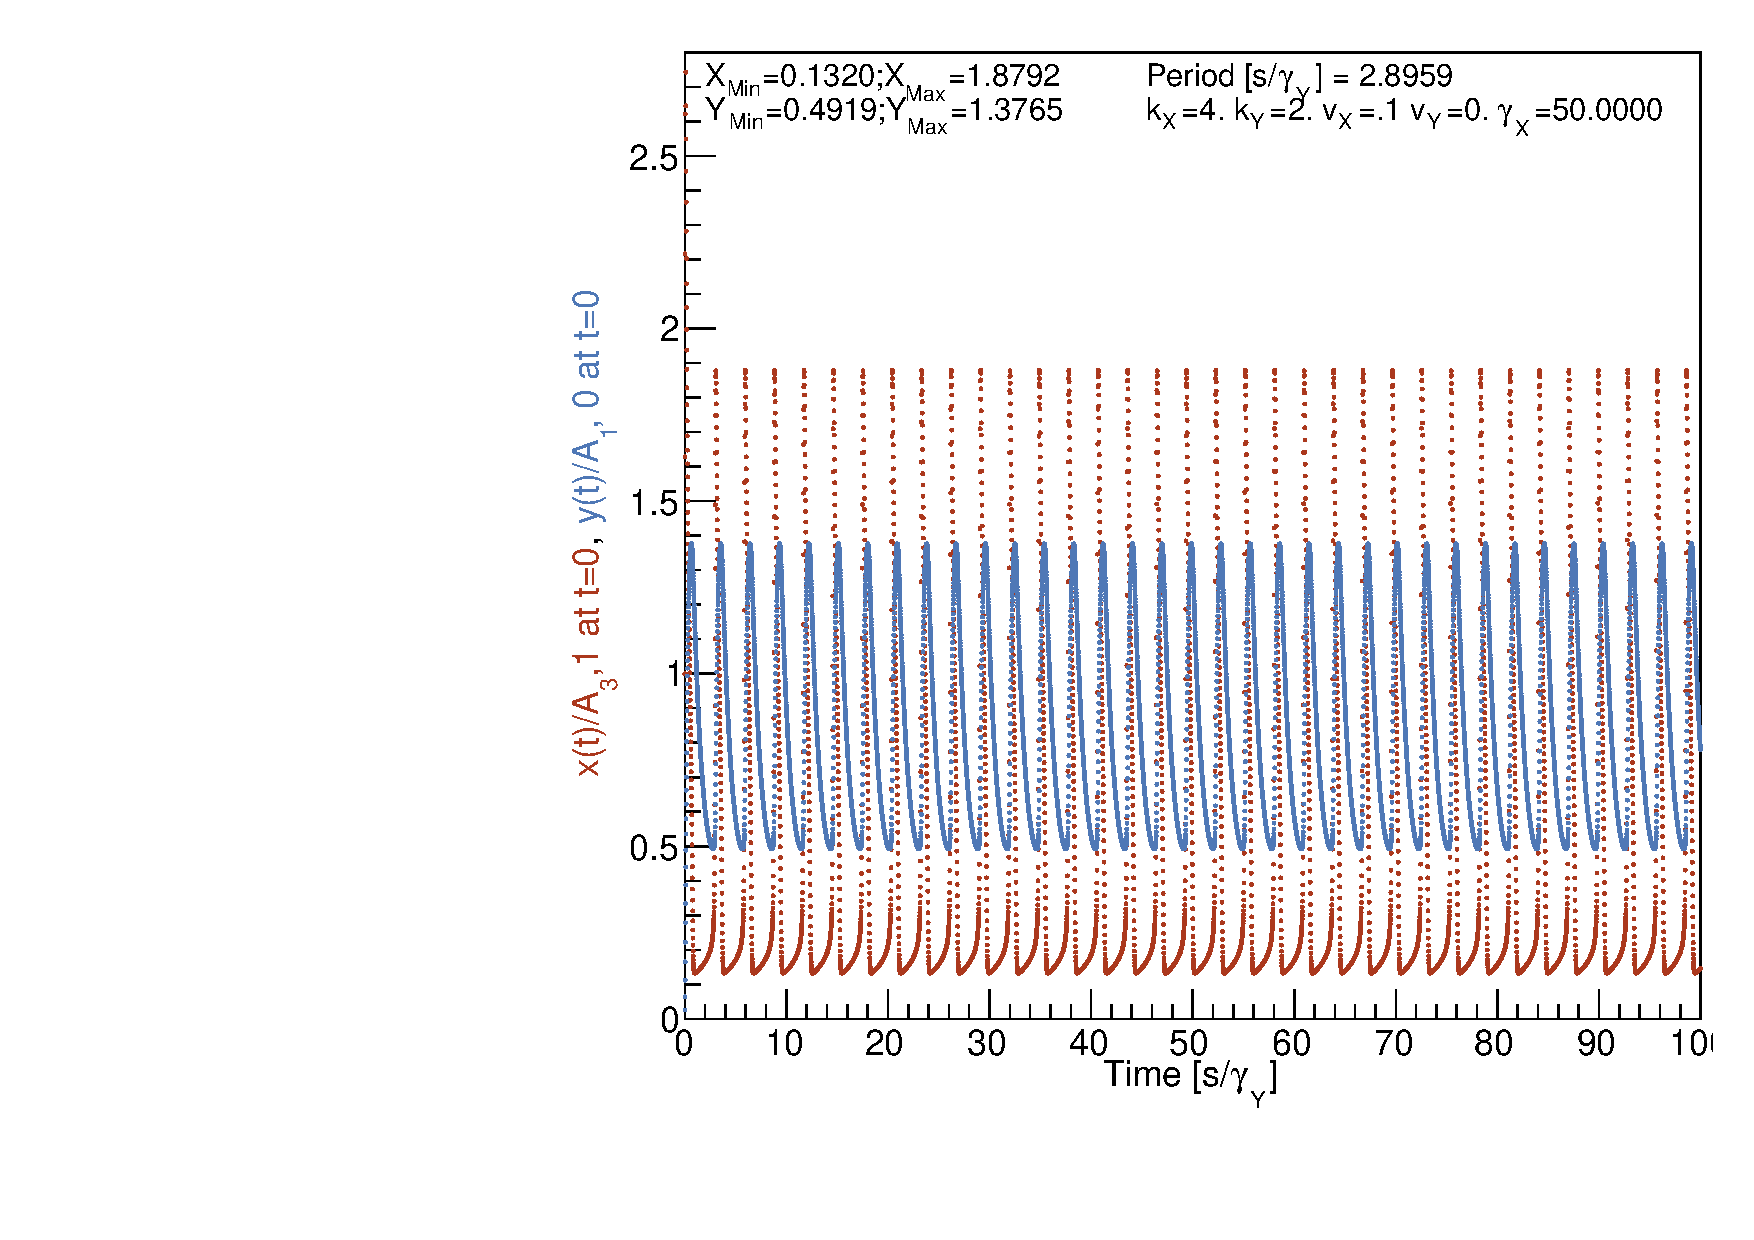
\includegraphics[width=.235\textwidth]{xy_Gamma50p0000_x1p0_y0p0_THigh100_c.pdf}
    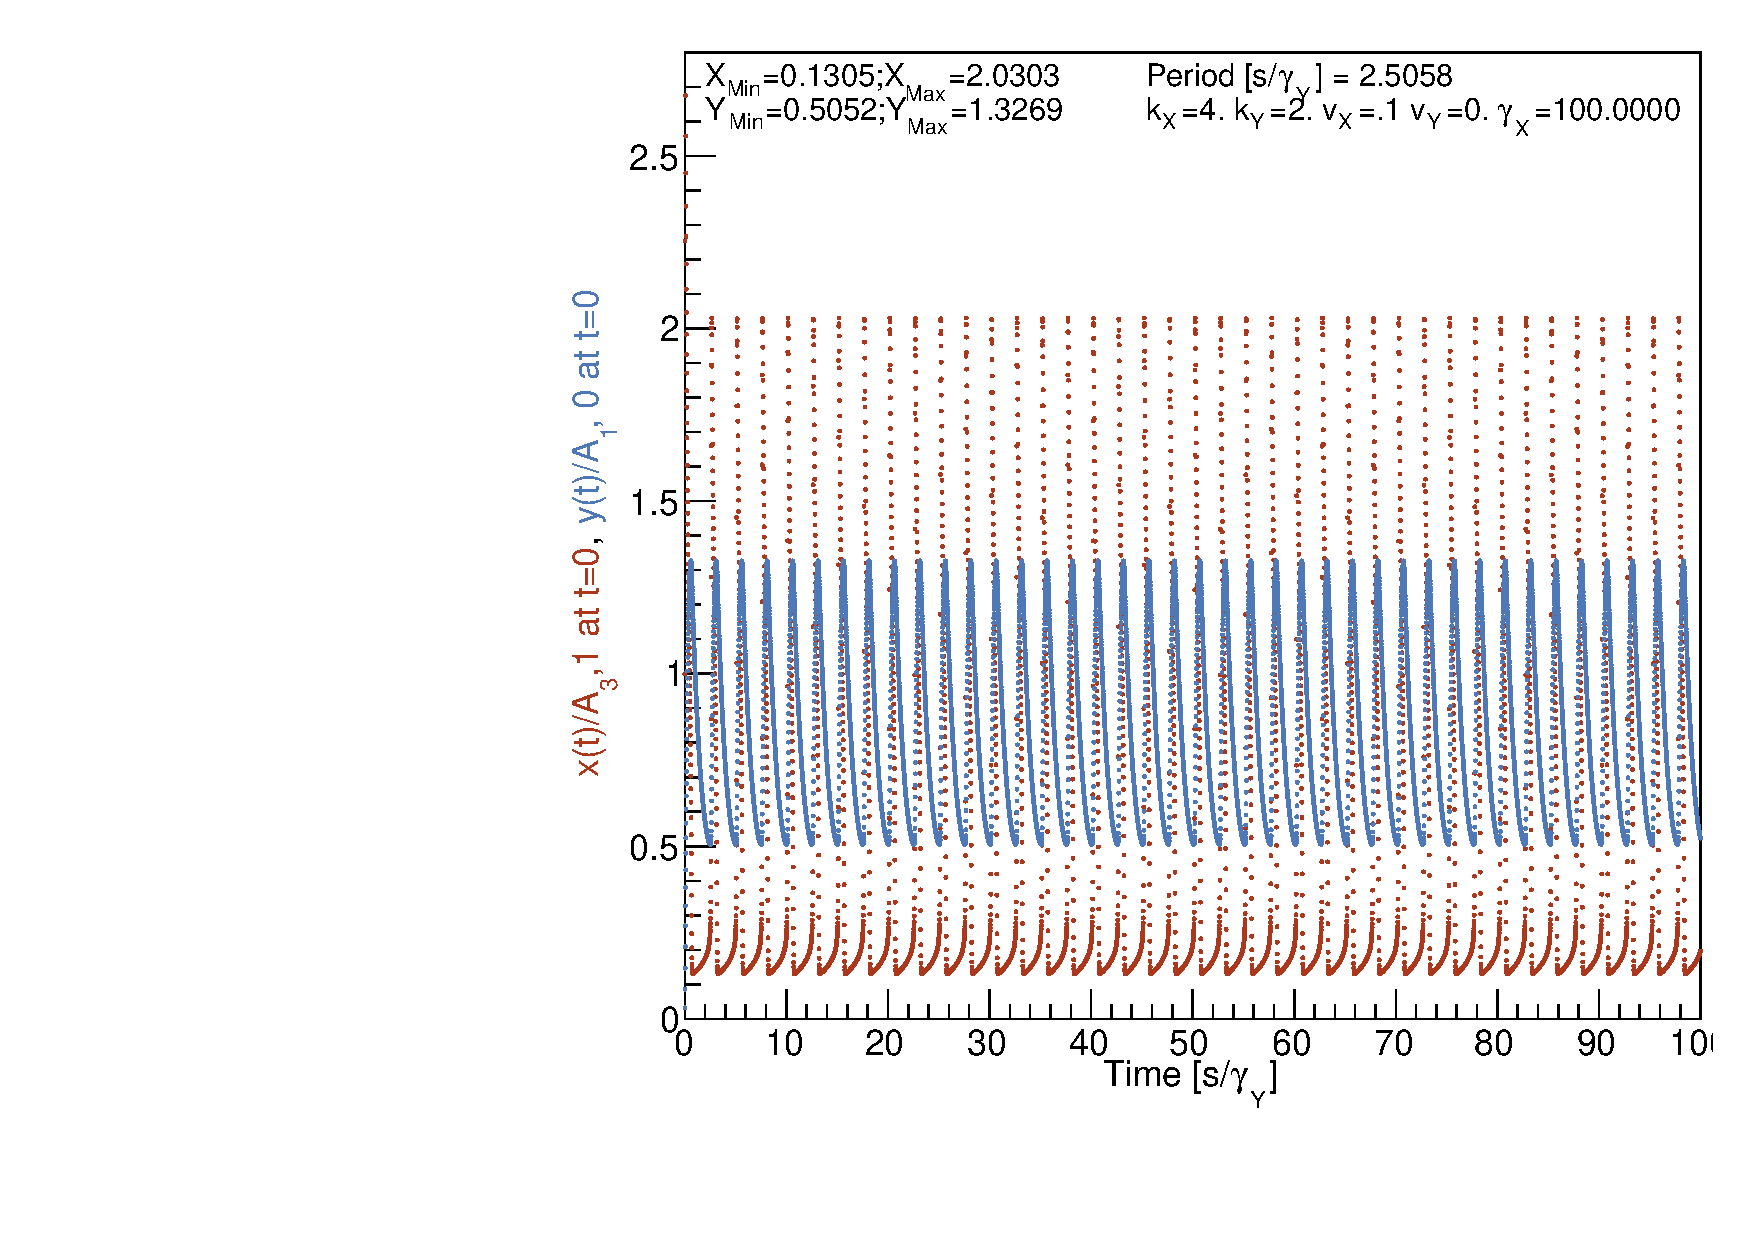
\includegraphics[width=.235\textwidth]{xy_Gamma100p0000_x1p0_y0p0_THigh100_c.pdf}
    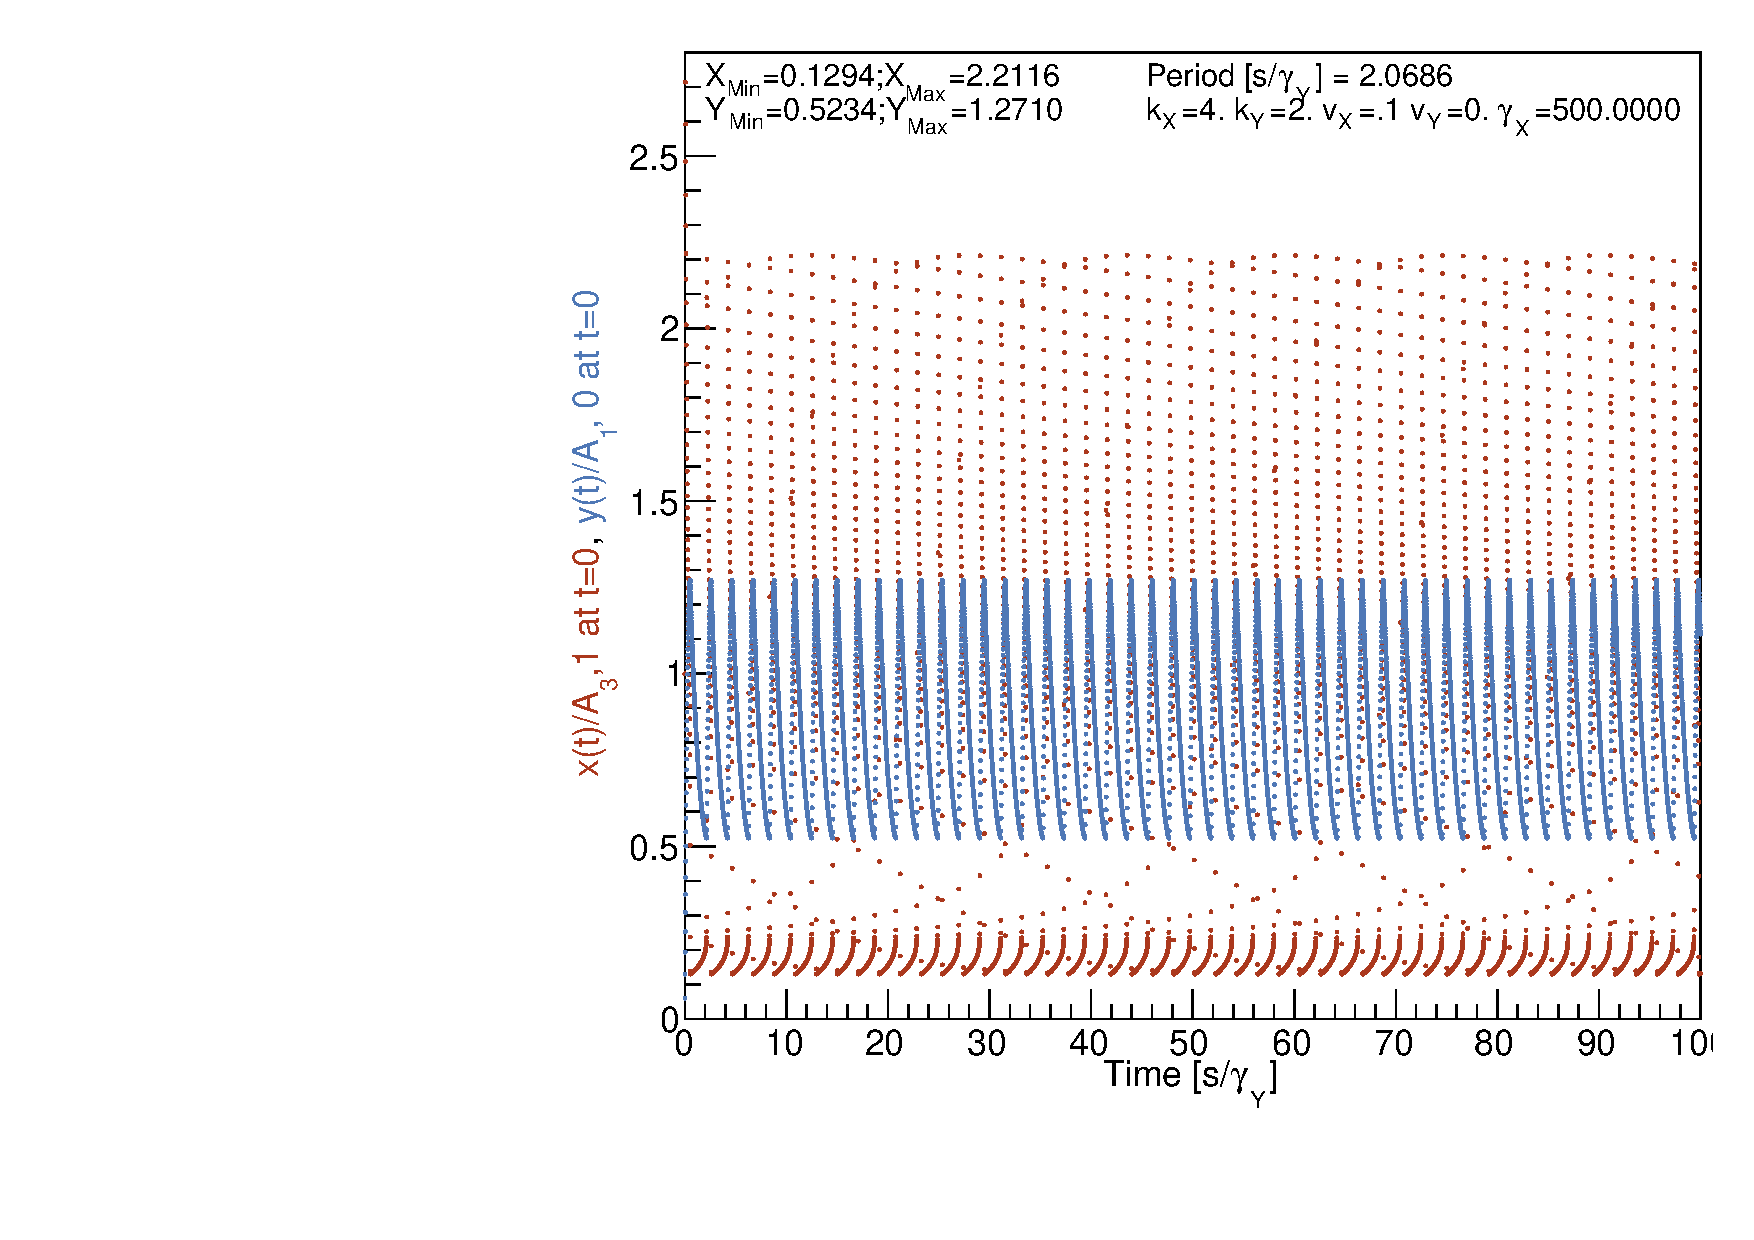
\includegraphics[width=.235\textwidth]{xy_Gamma500p0000_x1p0_y0p0_THigh100_c.pdf}
    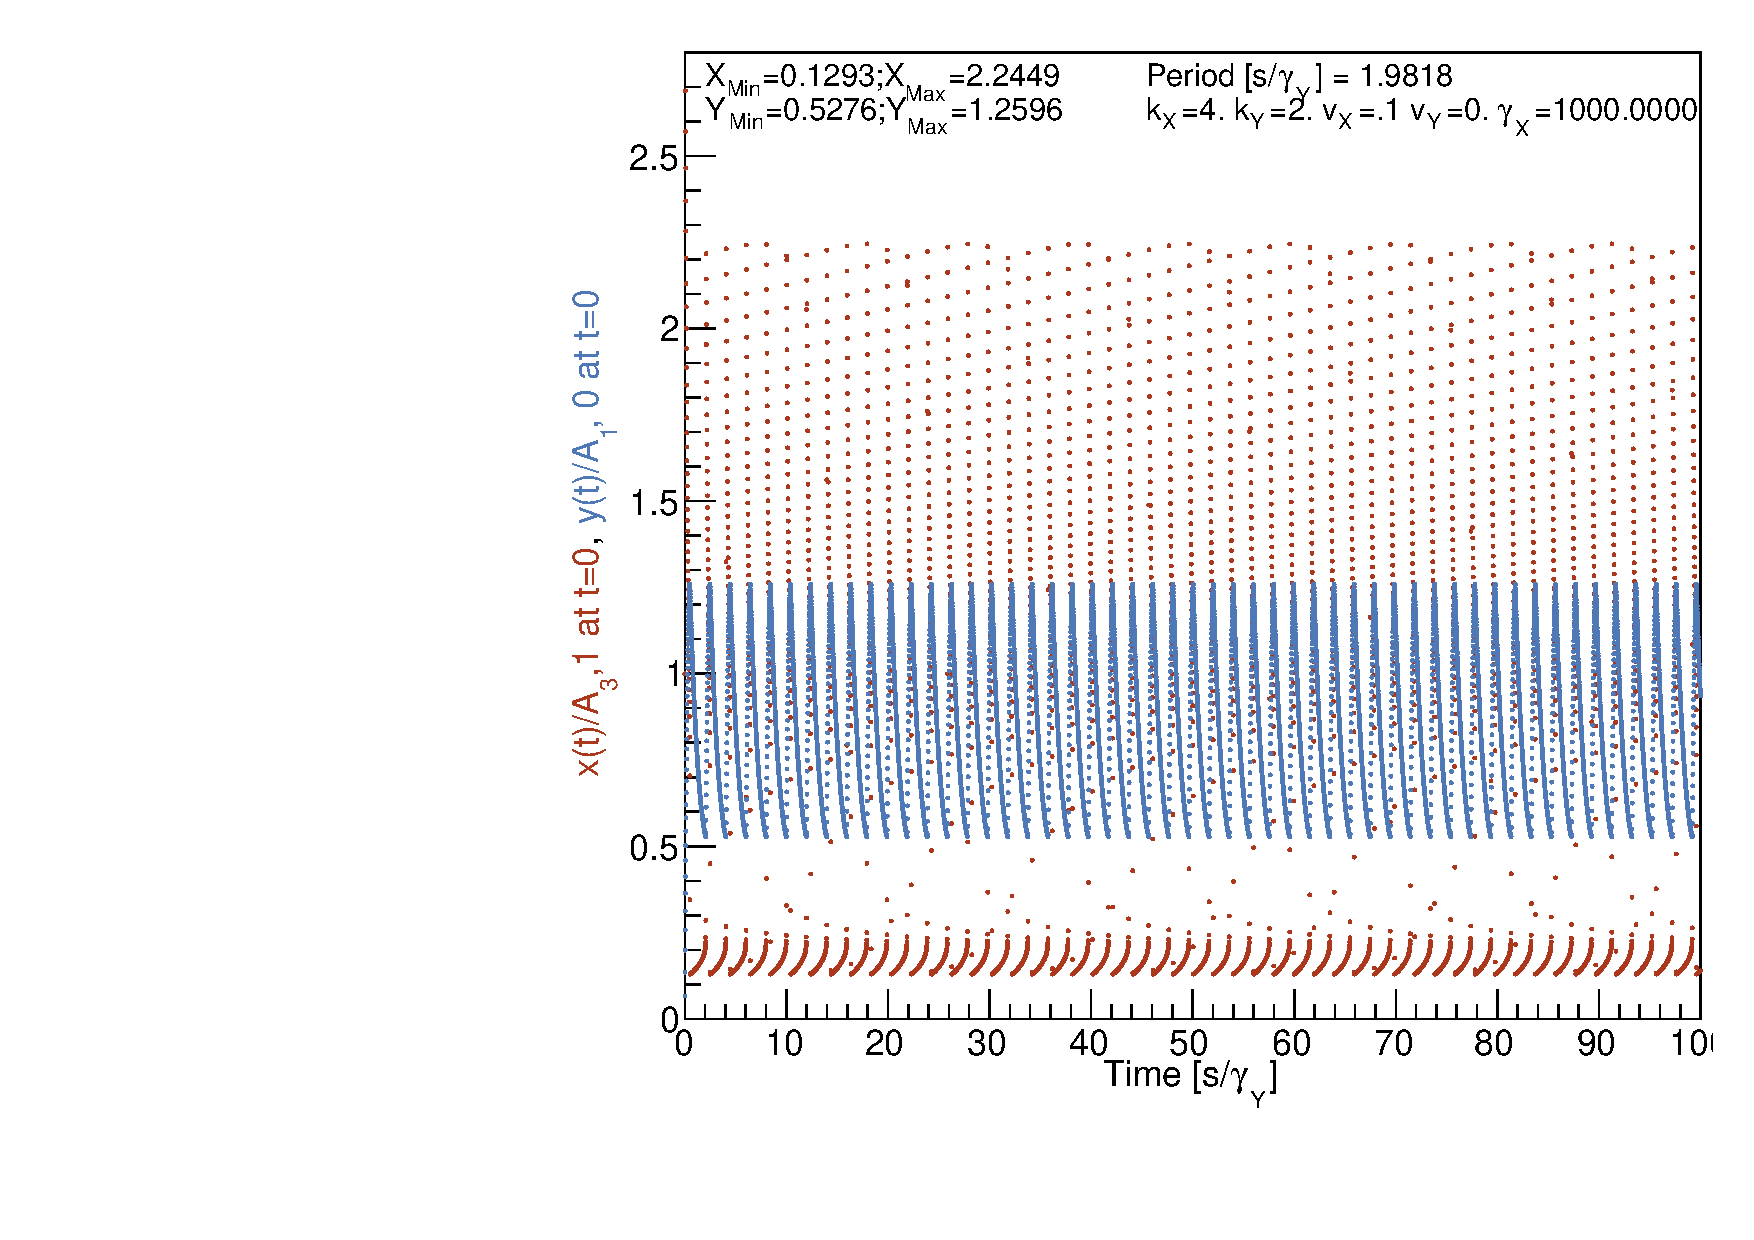
\includegraphics[width=.235\textwidth]{xy_Gamma1000p0000_x1p0_y0p0_THigh100_c.pdf}
    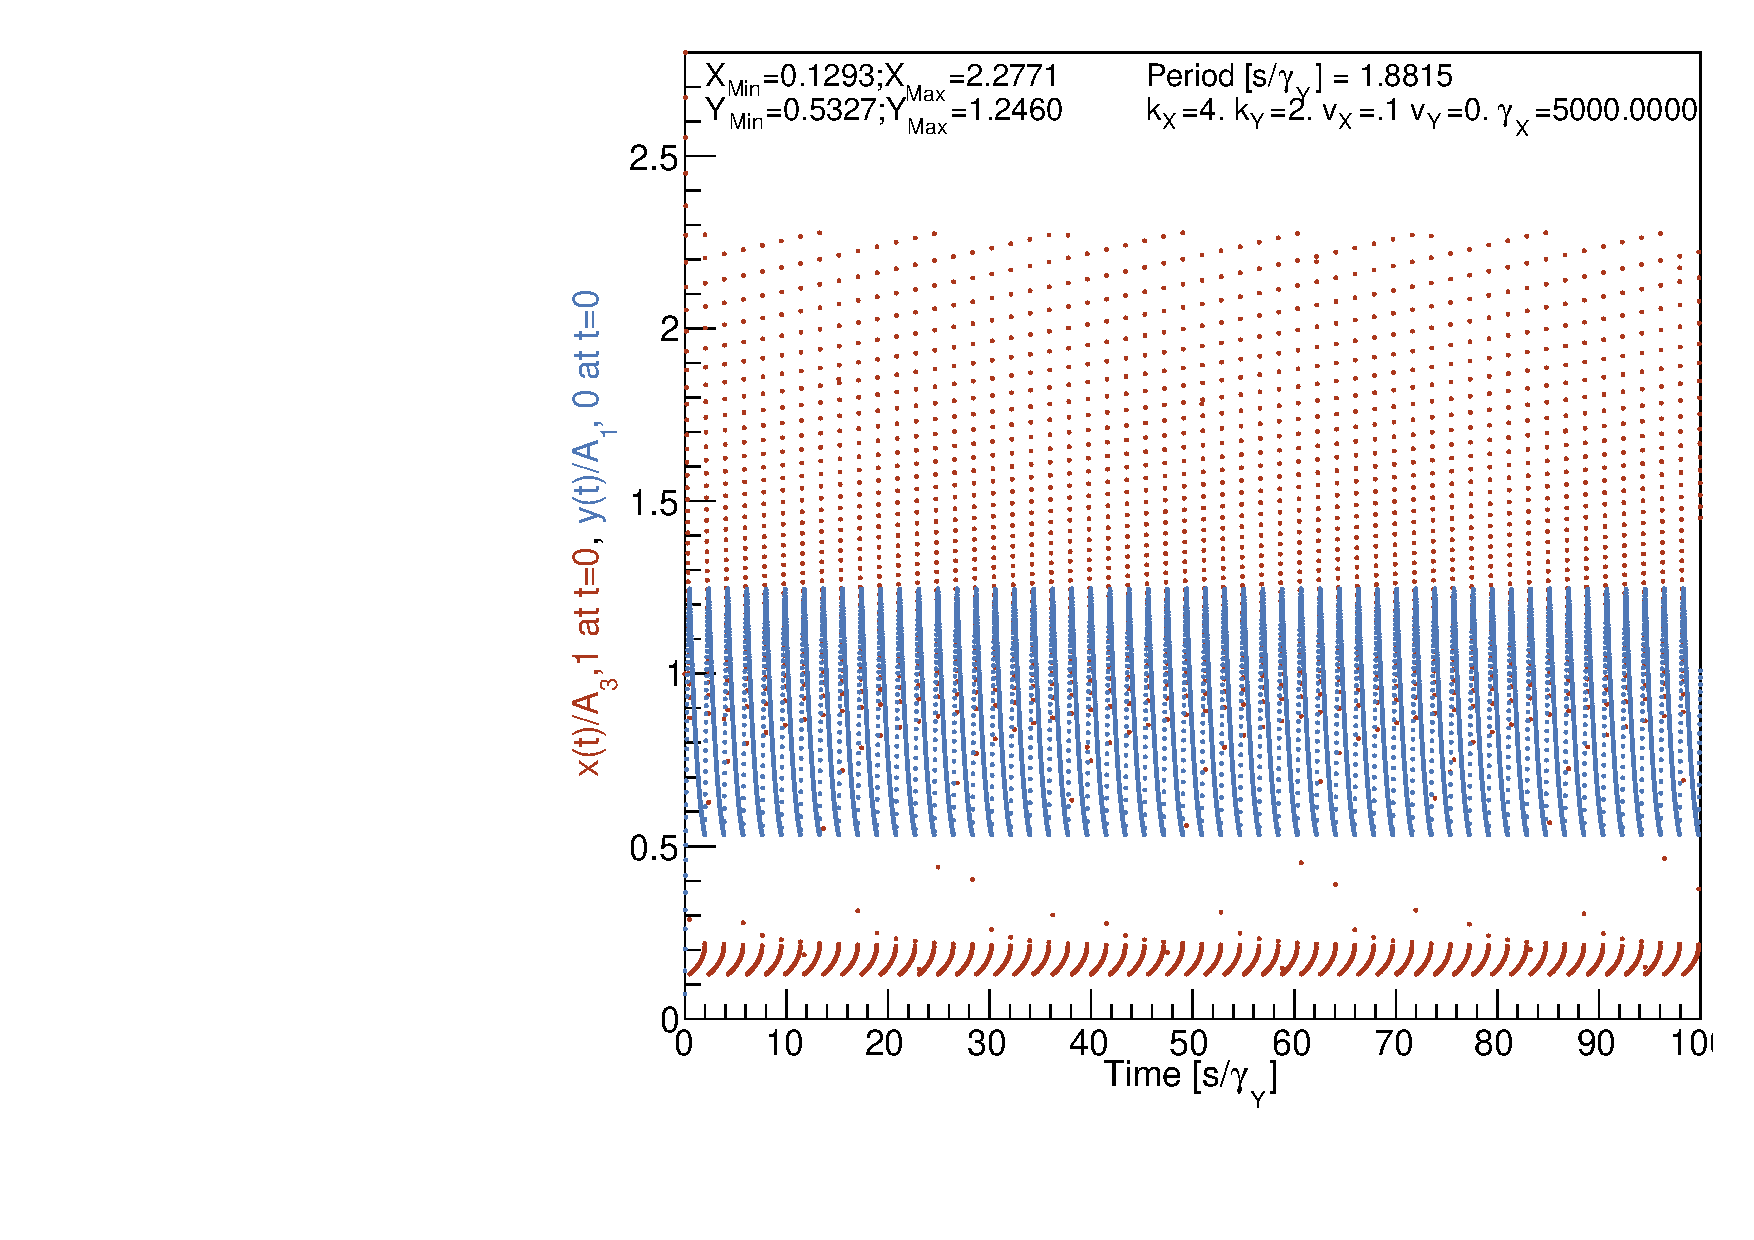
\includegraphics[width=.235\textwidth]{xy_Gamma5000p0000_x1p0_y0p0_THigh100_c.pdf}
    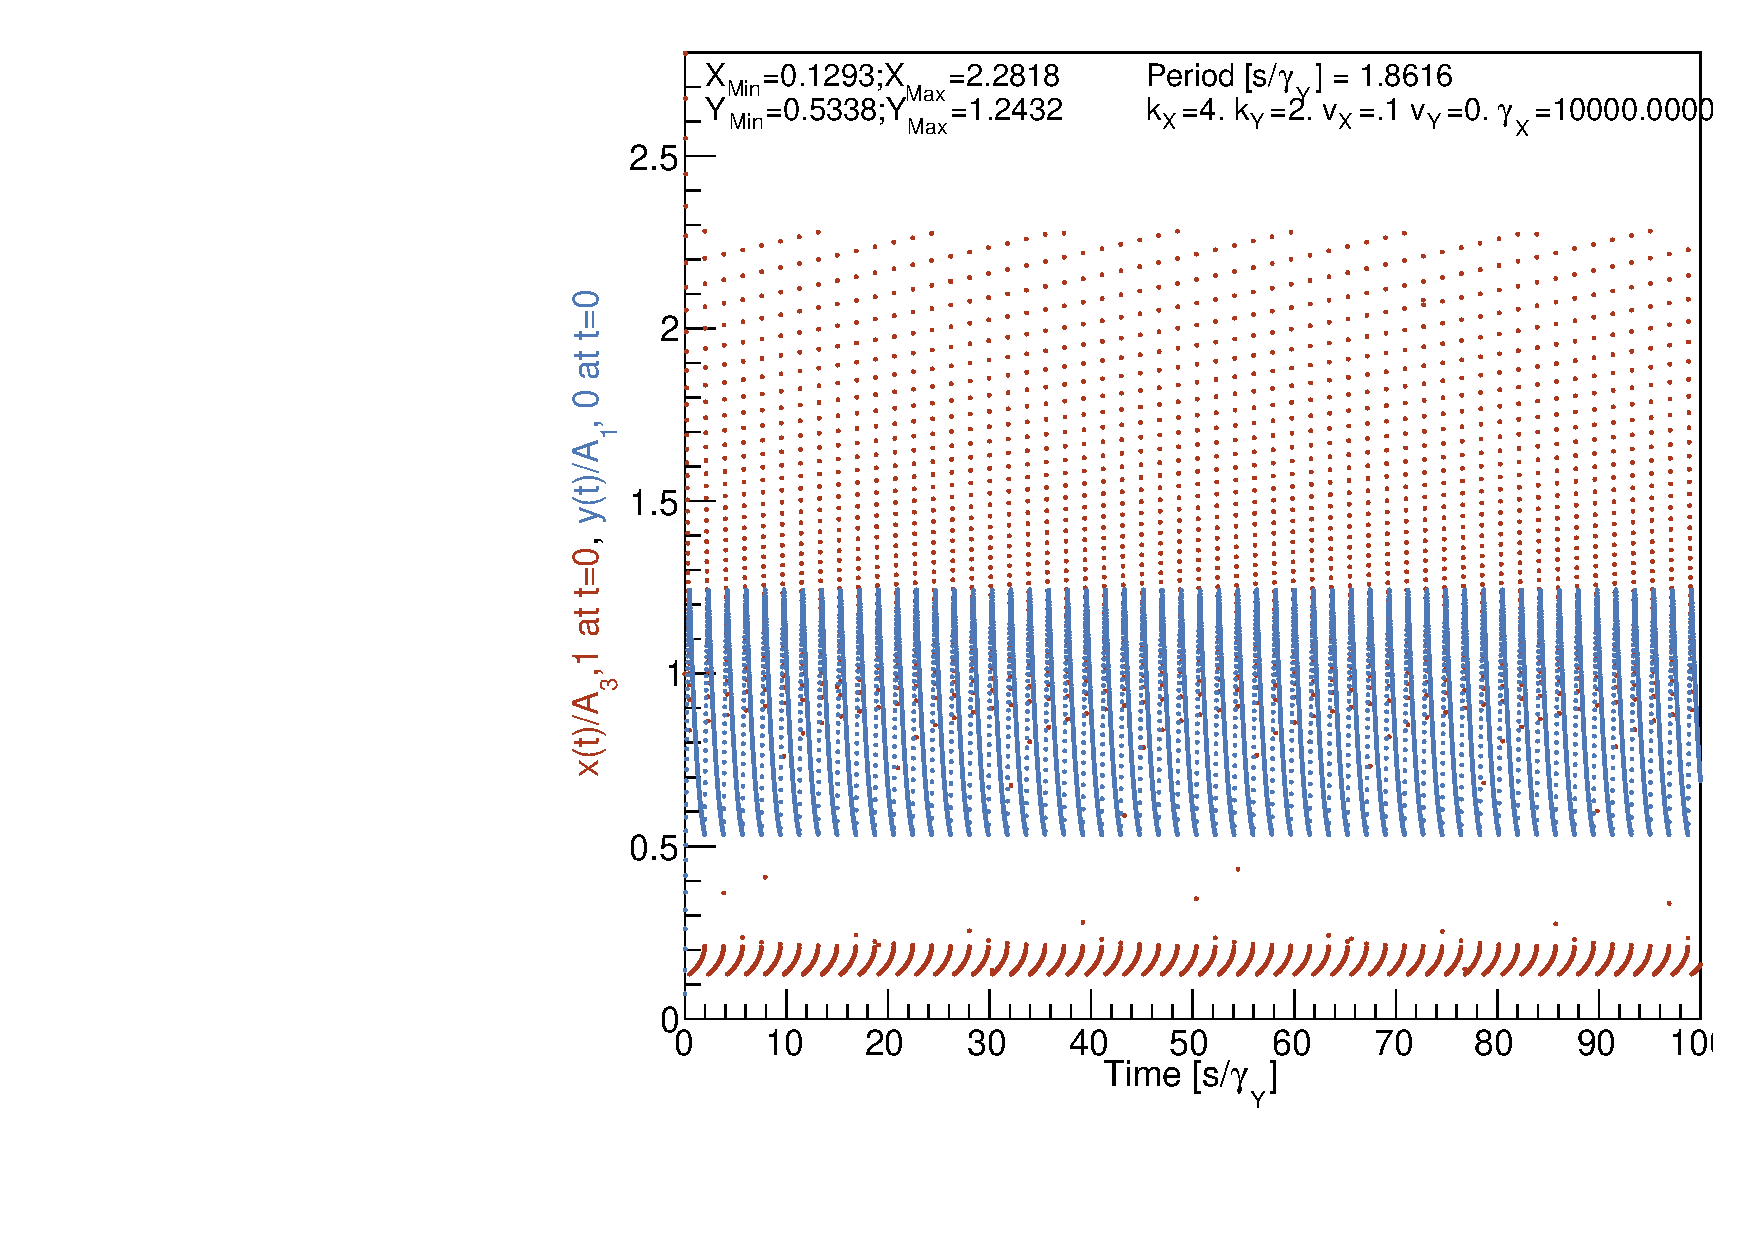
\includegraphics[width=.235\textwidth]{xy_Gamma10000p0000_x1p0_y0p0_THigh100_c.pdf}
    \caption{Simulation of system for initial condition $x=1,y=0$ thru 100 dimensionless timesteps for variation of $\gamma_{X}$. First panel is for decaying system to stable fixed point, rest are for different osciallating systems. Note as $\gamma_{X}$ increases, period decreases, amplited x increases, amplitude y decreases. All approach some asymtotic value.}
    \label{}
\end{figure}

\begin{figure}[H]
    \centering
    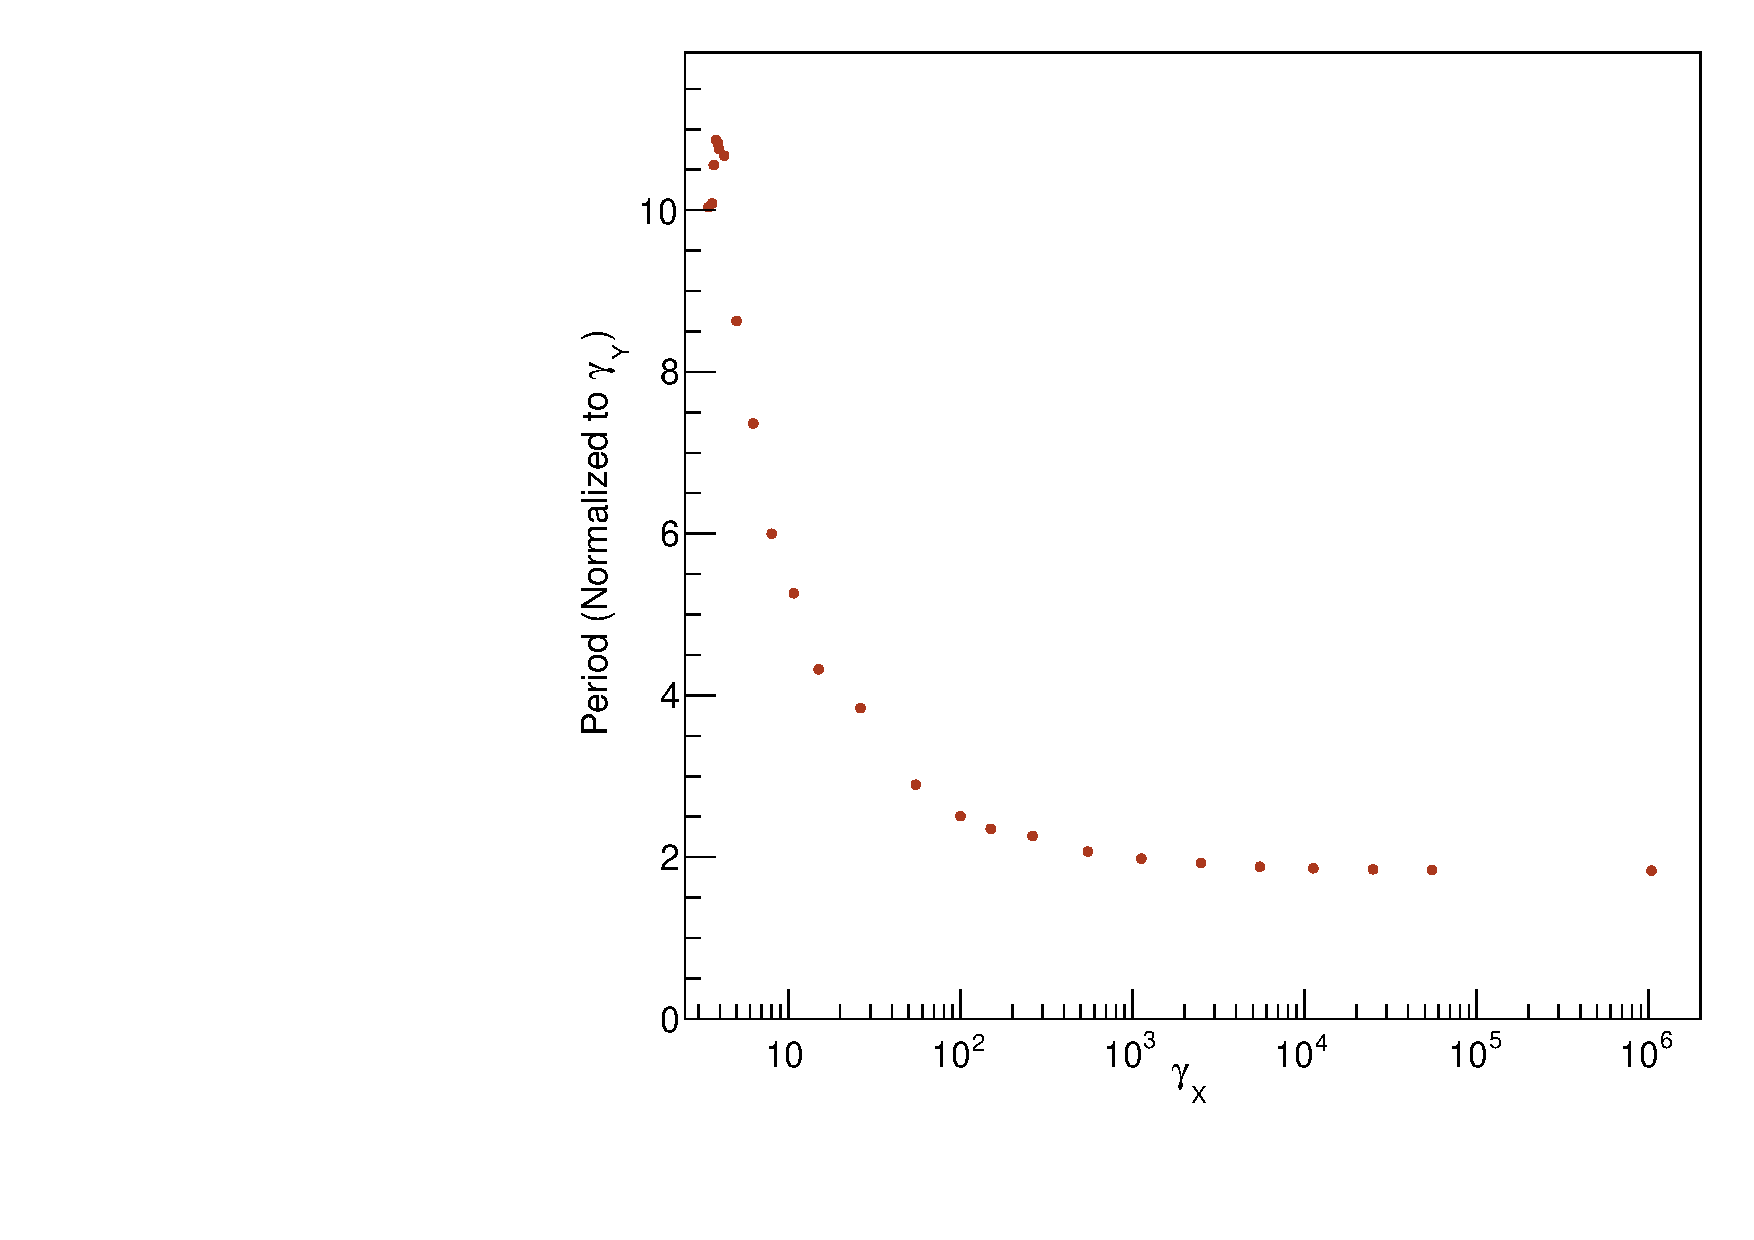
\includegraphics[width=.32\textwidth]{periodPerGamma_c.pdf}
    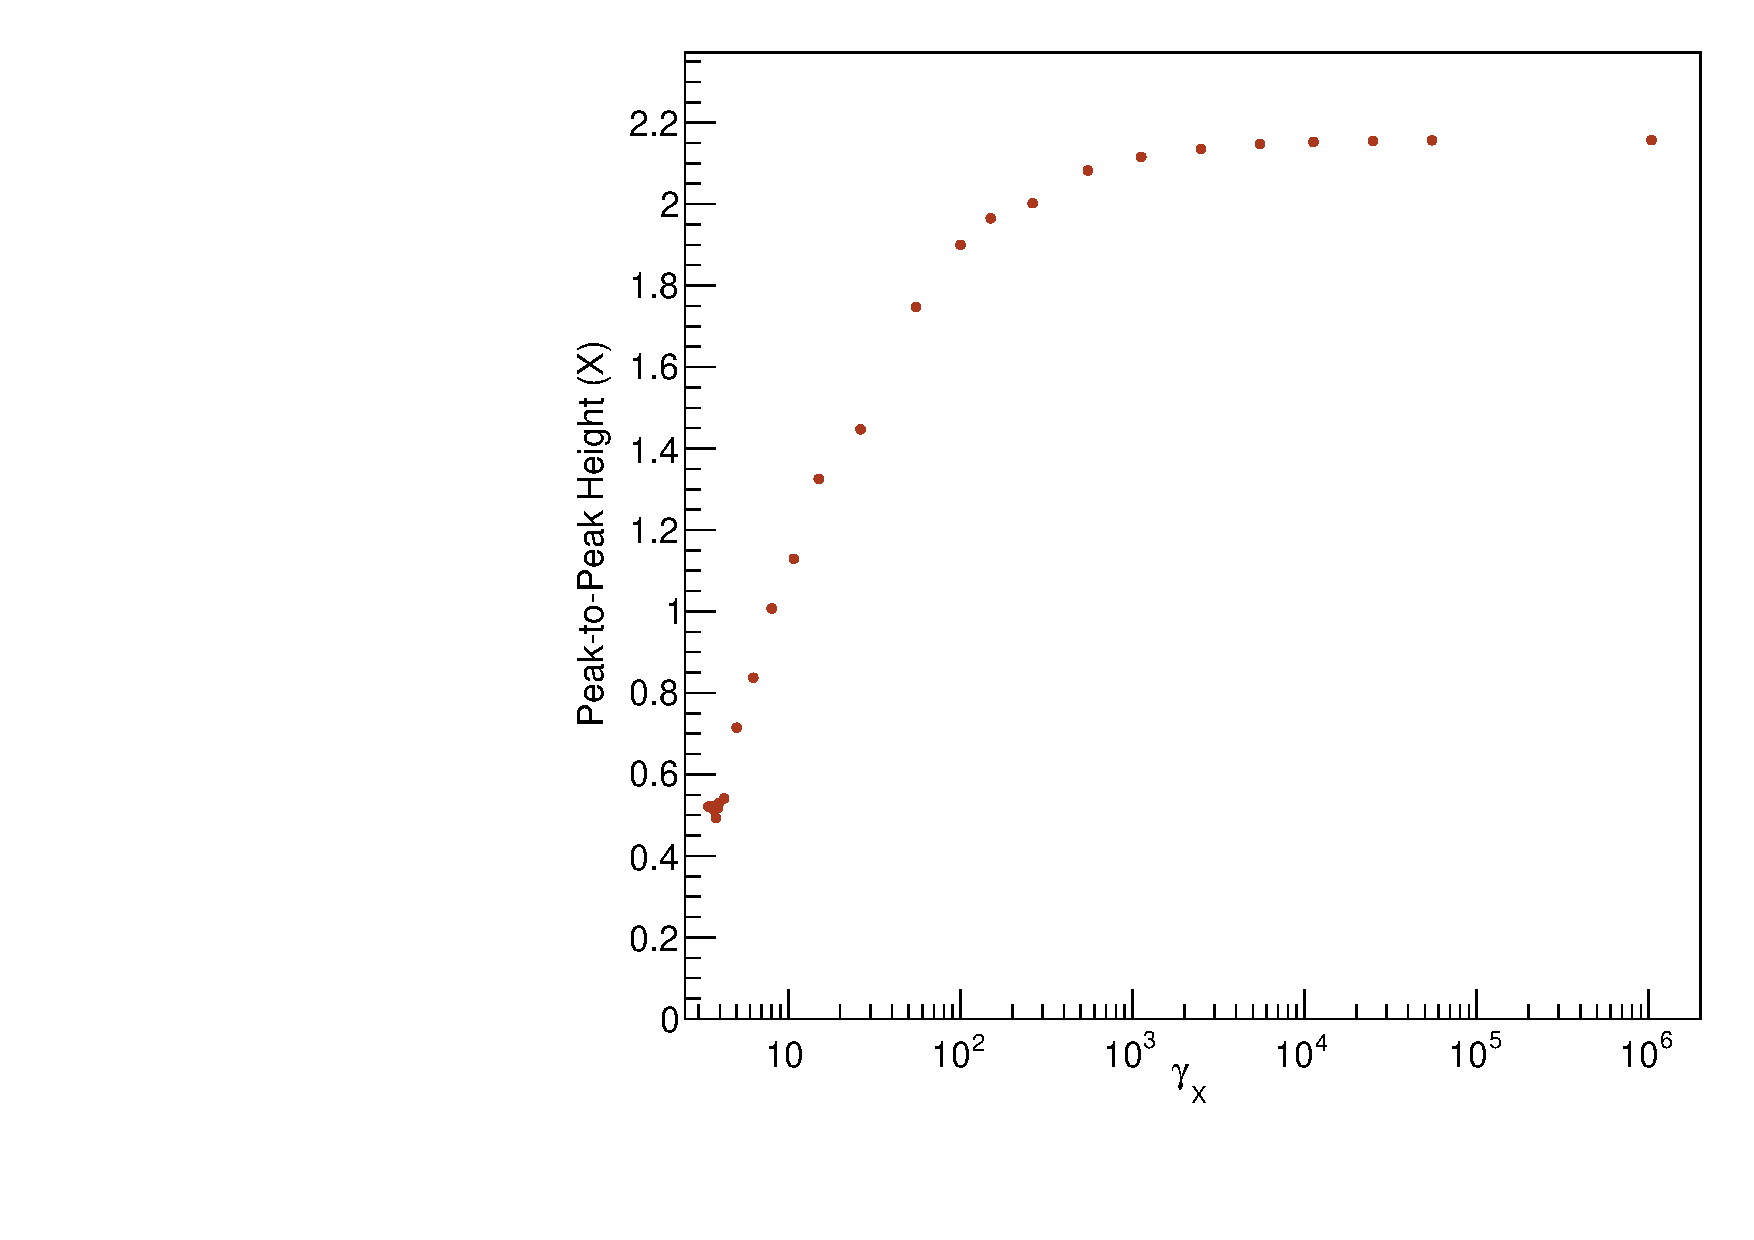
\includegraphics[width=.32\textwidth]{peakToPeakX_c.pdf}
    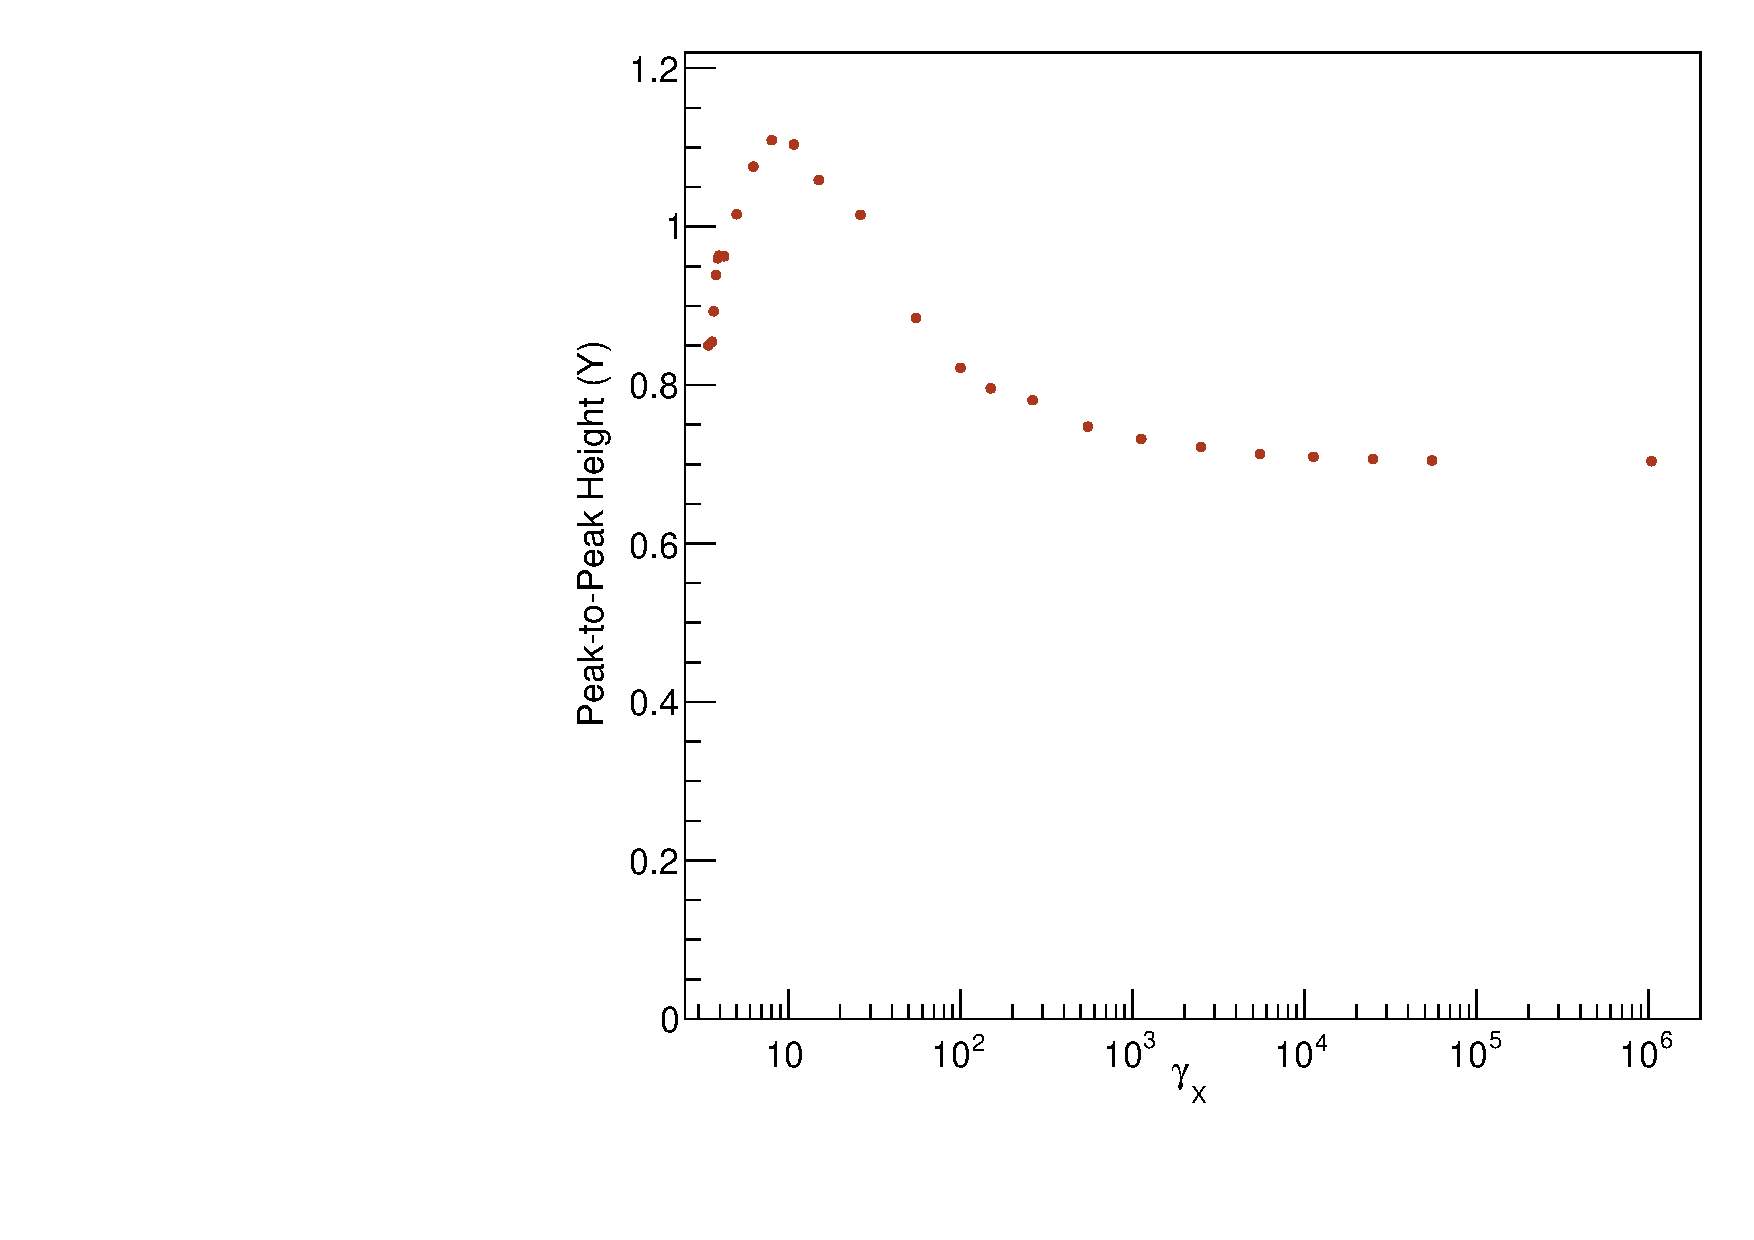
\includegraphics[width=.32\textwidth]{peakToPeakY_c.pdf}
    \caption{Period, amplitude X, amplitude Y, as a function of $\gamma_{X}$ in regime of sustained oscillations ($\gamma_{X} > 25/7$). Note that all three approach some asymtotic values as $\gamma_{X}$ goes to infinity. Note these are all dimensionless units, an all were evaluated at late time, far from region in time where initial conditions would modify stable oscillations.}
    \label{}
\end{figure}

\section{1.f.4}

System (B) belongs to class "relaxation oscillators", specifically a two-color network motif where X promotes Y and auto-regulates itself positively, but Y represses X. Examples in nature from Barkai and Leibler 2000 Nature article "Biological rhythyms: Circadian clocks limited by noise" are "positive elements (or activators, such as KaiA in Synechococcus, Wc1-2 in Neurospora, Clc and Cyc in Drosophila, and Clock and Bmal in mice) enhance the expression of negative elements (or repressors, such as KaiB and KaiC in Synechococcus, Frq in Neurospora, Tim and Per in Drosophila, and Tim and Per1,2 and 3 in mice)."

\end{document}

